%!TEX root = ../dissertation.tex
\chapter{Benchmark \textit{\&} Application}
\label{chap:06}

% \addcontentsline{toc}{section}{Introduction}
\Lettrine{Over} the previous chapters, several software developments have been presented. They try to fill different gaps in the multiscale modeling toolbox, be it the entry point to the funnel (GaudiMM) or to connect different stages down below (Tangram, OMMProtocol, Garleek$ \ldots $ ). In this chapter, several case studies where these programs have been used will be presented. Potential scenarios where they would be welcome will be also introduced as additional examples of applicability.

\section{GaudiMM as a versatile molecular modeling tool}

While GaudiMM's approach to molecular modeling can be daunting at first, once the key concepts are settled, configuring a calculation is straight-forward: it is a matter of which set genes and objectives to use. A particular combination of genes and objectives can be considered a \textit{recipe} that can be adjusted for one study and reused in similar ones just by changing the involved structures. The following \textit{recipes} will showcase common uses of GaudiMM.

\subsection{From standard to more exotic dockings}
% \addcontentsline{toc}{section}{GaudiMM as a versatile molecular modeling tool}

Classic protein-ligand docking studies devote to finding the correct orientation and position of a small molecule (the ligand) within the cavity of a bigger one (normally, a protein). It usually cares about supramolecular recognition only, which means that analyzed interactions are mostly non-bonded. As a result, covalent bonds and coordination geometries are usually left out. However, a lot of systems do exhibit this type of recognition. In our group, we work with metallodrugs and artificial enzymes, two fields where these phenomena play an important role. As a result, we had big interest in considering these aspects in our docking calculations.

In fact, GaudiMM was initially devised as an extensible protein-ligand tool, but later grew into a multi-purpose molecular modeling platform. The transition was smooth because the idea of docking can be further abstracted as simply \textit{finding structural geometries compatible with certain requirements}, which is in turn a very specific type of restrained optimization problems. In this section, we will present how GaudiMM can perform several types of docking.


\subsubsection{Flexible protein-ligand docking: a benchmark}
% \addcontentsline{toc}{subsection}{Ligand docking}

% \addcontentsline{toc}{subsubsection}{Protein-ligand docking}

GaudiMM capabilities for flexible protein-ligand docking were studied in its first publication,\cite{gaudimm} where it was benchmarked against three different datasets\footnote{GOLD dataset (100 entries), ChemScore dataset (166 entries) and the CCDC Astex dataset (305 entries). Available at \url{https://www.ccdc.cam.ac.uk/support-and-resources/downloads}.} using four genes and two objectives (see table \ref{table:docking-recipe} for more details).

All of the entries in each dataset were analyzed with full torsion flexibility on the ligand, which could move and rotate within 12 Å of the crystallographic position. The results were analyzed considering the best RMSD of each calculation against the crystallographic reference structure. The correct binding pose was considered successfully reproduced if the RMSD was under than 3.0 Å. Despite not being the target usage of GaudiMM, the recipe reported success rates of up to 57.6$\%$ (see table \ref{table:docking-benchmark}), a value comparable to several works in the literature.\cite{pagadala2017software} With more efforts directed at optimizing the exploration stage (especially the variation operators on torsion and orientation), the number of hits would highly increase and compete with other docking software.

\begin{table}[hbtp]
	\caption{Recipe applied in the docking benchmark}
	\label{table:docking-recipe}
	\footnotesize
	\newcolumntype{R}{>{\hsize=.25\hsize\raggedleft\arraybackslash}X}%
	\newcolumntype{L}{>{\hsize=.75\hsize\raggedright\arraybackslash}X}%
	\newcommand{\tableheading}[1]{\multicolumn{2}{c}{\textsc{#1}}}
	\begin{tabularx}{\textwidth}{RL}
		\toprule
		%row no:1
		\tableheading{Genes}\\
		\toprule
		%row no:2
		\texttt{Molecule} & Load the protein \\
		\midrule
		\texttt{Molecule} & Load the ligand \\
		\midrule
		\texttt{Torsion} & Explore internal flexibility of the ligand \\
		\midrule
		\texttt{Search} & Move the ligand within 12 Å of its starting point \\
		\toprule
		%row no:4
		\tableheading{Objectives}\\
		\toprule
		%row no:5
		\texttt{Contacts} & Minimize steric clashes \\
		\midrule
		\texttt{Contacts} & Maximize hydrophobic interactions (target distance thresholds adapted) \\
		\midrule
		%row no:6
		\texttt{LigScore} & Minimize scoring function value \\
		\bottomrule
	\end{tabularx}
\end{table}

%%%%%%%%%%%%%%%%%%%% Table No: 1 starts here %%%%%%%%%%%%%%%%%%%%


\begin{table}[H]
	\cprotect\caption[Success rate of GaudiMM in a docking benchmark]{Success rate\textsuperscript{†} of a LigScore GaudiMM recipe against four benchmark datasets.}
	\label{table:docking-benchmark}
	\centering
	\footnotesize
	\newcolumntype{R}{>{\raggedleft\arraybackslash}X}%
	\newcolumntype{C}{>{\centering\arraybackslash}X}%
	\begin{tabularx}{\textwidth}{CCCC}
		\toprule
		\multirow{2}{*}{RMSD\textsubscript{max}} & \multicolumn{3}{c}{Benchmarked dataset}            \\ \cmidrule(l){2-4}
								 & CCDC Astex\textsuperscript{a} & GOLD\textsuperscript{b}    & ChemScore\textsuperscript{c}  \\ \midrule
		2.5 \AA                  & 41.64\%    & 45.45\% & 45.45\%  \\ \midrule
		3.0 \AA                  & 51.80\%    & 57.58\% & 51.52\%  \\ \bottomrule
		\multicolumn{4}{p{0.9\textwidth}}{\textsuperscript{†}Success was considered if at least one solution with LigScore score < 0 had an RMSD against the XRD structure within the given threshold. \textsuperscript{a}305 entries. \textsuperscript{b}100 entries. \textsuperscript{c}166 entries.} \\
	\end{tabularx}
 \end{table}


\subsubsection{Covalently restrained docking of several ligands at once}
\label{section:multidocking}
% \addcontentsline{toc}{subsubsection}{Covalently restrained docking}

As explained, sometimes there is an interest beyond non-bonded recognition, like when the ligand is covalently attached to some part of the protein. While there is no specific gene to implement a covalent bond, it can be mimicked through a \texttt{Search} gene configured to perform only rotation (translation can be disabled if $search~radius=0$). As this null \texttt{Search} gene will consider all possible rotations from that point, an \texttt{Angle} objective between the involved atoms in the covalent bond is recommended so that the resulting rotation matches the expected geometry of the new bond.\footnote{For example, for a carbon atom: $109.5^{\circ}$ for \textit{sp\textsuperscript{3}}, $120^{\circ}$ for \textit{sp\textsuperscript{2}}, $180^{\circ}$ for \textit{sp\textsuperscript{1}}} If more covalent interactions are needed, those can be modeled with a \texttt{Distance} objective set to bring the involved atoms within their covalent range (automatically calculated with the \textit{covalent} keyword).

Additionally, taking advantage of the fact that genes and objectives can be instantiated multiple times,\footnote{For example, in the previous sections, protein and ligand molecules were loaded with separate instances of the \texttt{Molecule} gene} two or more \texttt{Molecule} genes can be set to open one ligand each. The compounds will be loaded simultaneously and they will compete to find their place in the protein(s). For this strategy to work, any related genes that are acting on the ligands (i.e. \texttt{Search} or \texttt{Torsion}) must be replicated accordingly.

This strategy allows competitive multi-ligand docking, something which is directly not possible in most docking software suites. It is true that it can be mimicked by performing sequential studies, in which the first ligand is docked separately and then the resulting solutions (protein \textit{plus} first ligand) are fed as the host structure of the second ligand. However, in that context they would not be competing for the protein space simultaneously, per se: one of them has \textit{priority} access. The procedure should be repeated to consider all possible orderings in order to be fair. With GaudiMM, this is not necessary since they are competing during the whole simulation.

Both concepts ---covalent bond emulation and competitive docking--- were tested during the design of an artificial metalloenzyme featuring a copper-containing phenanthroline cofactor covalently attached at the position M89C of the dimeric \textit{Lactococcal multidrug resistance Regulator} (LmrR) protein. While the final structures in that work (manuscript under preparation) propose a single cofactor, having two ligands simultaneously attached to both monomers was also considered at the beginning of the study. To assess that possibility, a GaudiMM calculation was set up to see if two covalently attached ligands can fit within the dimeric interface (see table \ref{table:phn-recipe} for details).

\begin{table}[hbtp]
	\caption{Recipe applied for the LmrR competitive docking calculations}
	\label{table:phn-recipe}
	\footnotesize
	\newcolumntype{R}{>{\hsize=.25\hsize\raggedleft\arraybackslash}X}%
	\newcolumntype{L}{>{\hsize=.75\hsize\raggedright\arraybackslash}X}%
	\newcommand{\tableheading}[1]{\multicolumn{2}{c}{\textsc{#1}}}
	\begin{tabularx}{\textwidth}{RL}
		\toprule
		%row no:1
		\tableheading{Genes}\\
		\toprule
		%row no:2
		\texttt{Molecule} & Load the LmrR protein (dimer) \\
		\midrule
		\texttt{Molecule} & Load a copy of the Cu-Phn cofactor (ligand) and anchor it into position 89 of monomer A \\
		\midrule
		\texttt{Molecule} & Load a copy of the Cu-Phn cofactor (ligand) and anchor it into position 89 of monomer B \\
		\midrule
		\texttt{Torsion} & Explore internal flexibility of the ligand A \\
		\midrule
		\texttt{Torsion} & Explore internal flexibility of the ligand A \\
		\midrule
		\texttt{Search} & Allow free rotation of ligand A from its anchor, but no translation ($radius=0$) \\
		\toprule
		\texttt{Search} & Allow free rotation of ligand B from its anchor, but no translation ($radius=0$) \\
		\toprule
		%row no:4
		\tableheading{Objectives}\\
		\toprule
		%row no:5
		\texttt{Contacts} & Minimize steric clashes \\
		\midrule
		\texttt{Contacts} & Maximize hydrophobic interactions (target distance thresholds adapted) \\
		\midrule
		%row no:6
		\texttt{Angle} & Force an angle of $109.5^\circ$ in anchor point of ligand A \\
		\midrule
		%row no:6
		\texttt{Angle} & Force an angle of $109.5^\circ$ in anchor point of ligand B \\
		\midrule
		\texttt{DSX} & Maximize docking scoring function to select stabilizing interactions \\
		\midrule
		\texttt{Solvation} & Minimize solvent-accessible surface area (SASA) so the ligands are forced to interact within the protein rift instead of avoiding clashes in the exterior area \\
		\bottomrule
	\end{tabularx}
\end{table}

Under this scheme, several satisfactory solutions were obtained (see fig. \ref{fig:phenanthroline}) and submitted to a MD simulation to test their stability. Unfortunately, the trajectories did not report any long-lasting interaction between the ligands inside the protein and this alternative model was discarded. It must be highlighted that no experimental information was available besides the protein structure. With GaudiMM, new models could be obtained which, at least, suggested an idea on how this systems could be.

\begin{figure}[H]
	\begin{Center}
		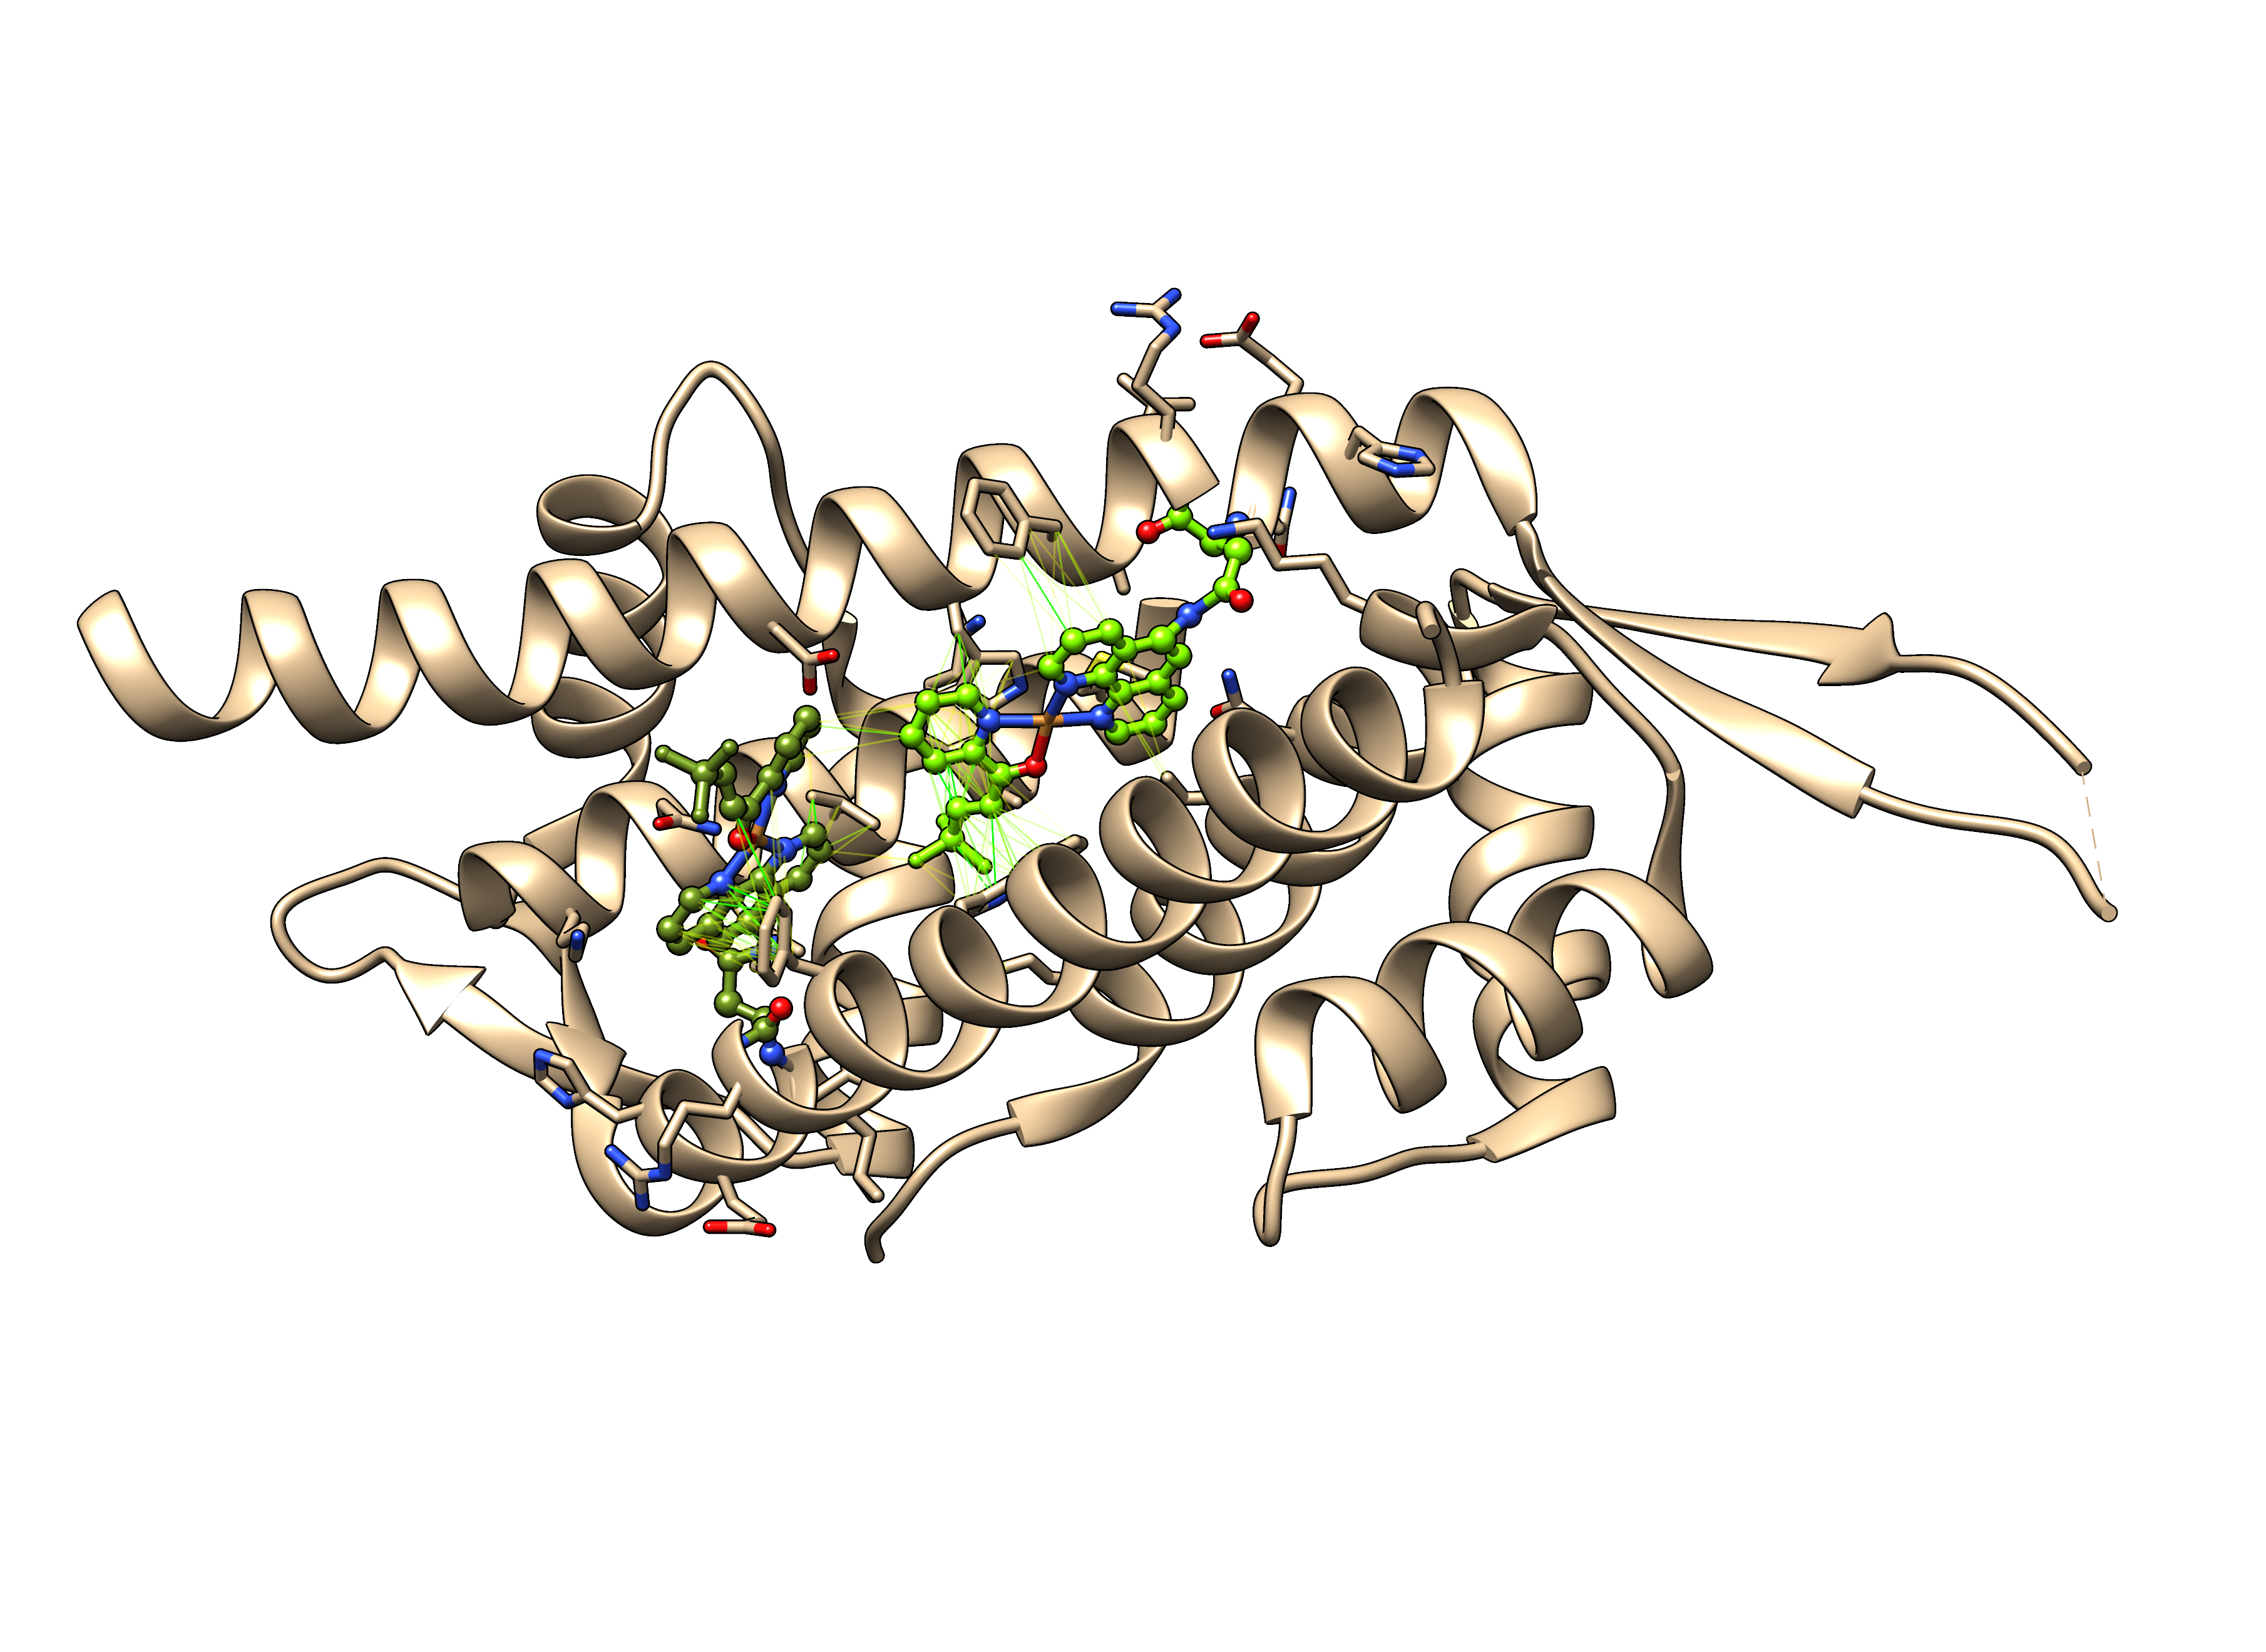
\includegraphics[width=\textwidth]{./figures/06/dual_phn.png}
	\end{Center}
	\caption[Proposed Cu-containing phenanthroline cofactors]{One the candidate structures proposed by GaudiMM. The two Cu-containing phenanthroline cofactors (in green) were covalently attached to position 89 in both monomers of the dimeric LmrR protein. While the results were promising, the subsequent MD simulation proved that that particular conformation did not feature long-lasting interactions.}
	\label{fig:phenanthroline}
\end{figure}

\subsubsection{Dynamic docking \& linker-length optimization}
% \addcontentsline{toc}{subsection}{Molecular design: linker-length optimization}
\label{section:dibiotin-linker-length-optimization}

The LmrR system is part of one of the most successful strategies to bring new stereoselective reactivities into existing enzymes: introducing cofactors that can anchor to the host and expose the catalytic region in a particular way. The anchoring can take place via a covalent bond (like in the previous case), but it can also be established through non-bonded interactions. In the latter case, biotin-derived cofactors have been particularly popular due to its high affinity to avidin and its bacterial counterpart, streptavidin, much easier to produce.

Streptavidin is composed of four monomers arranged as a dimer of dimers, each able to host a biotin molecule (see fig. \ref{fig:streptavidin}). One possible strategy to fix a catalytic cofactor within the protein is to build a dibiotin derivative that could anchor to both binding sites simultaneously, holding the catalytic cofactor in the dimeric interface. This way, only one side of the cofactor is exposed to the medium, bringing higher enantioselectivity.

Ward and collaborators were trying to build this hypothetical ligand, but simply bonding the copper cofactor to one biotin on each side would not result in a compound able to reach both sites: a linker or spacer was needed to connect the biotins to the cofactor. The question is: which is the optimal length so the resulting ligand reaches both sites? This is where GaudiMM could help.

\begin{figure}[H]
	\begin{Center}
		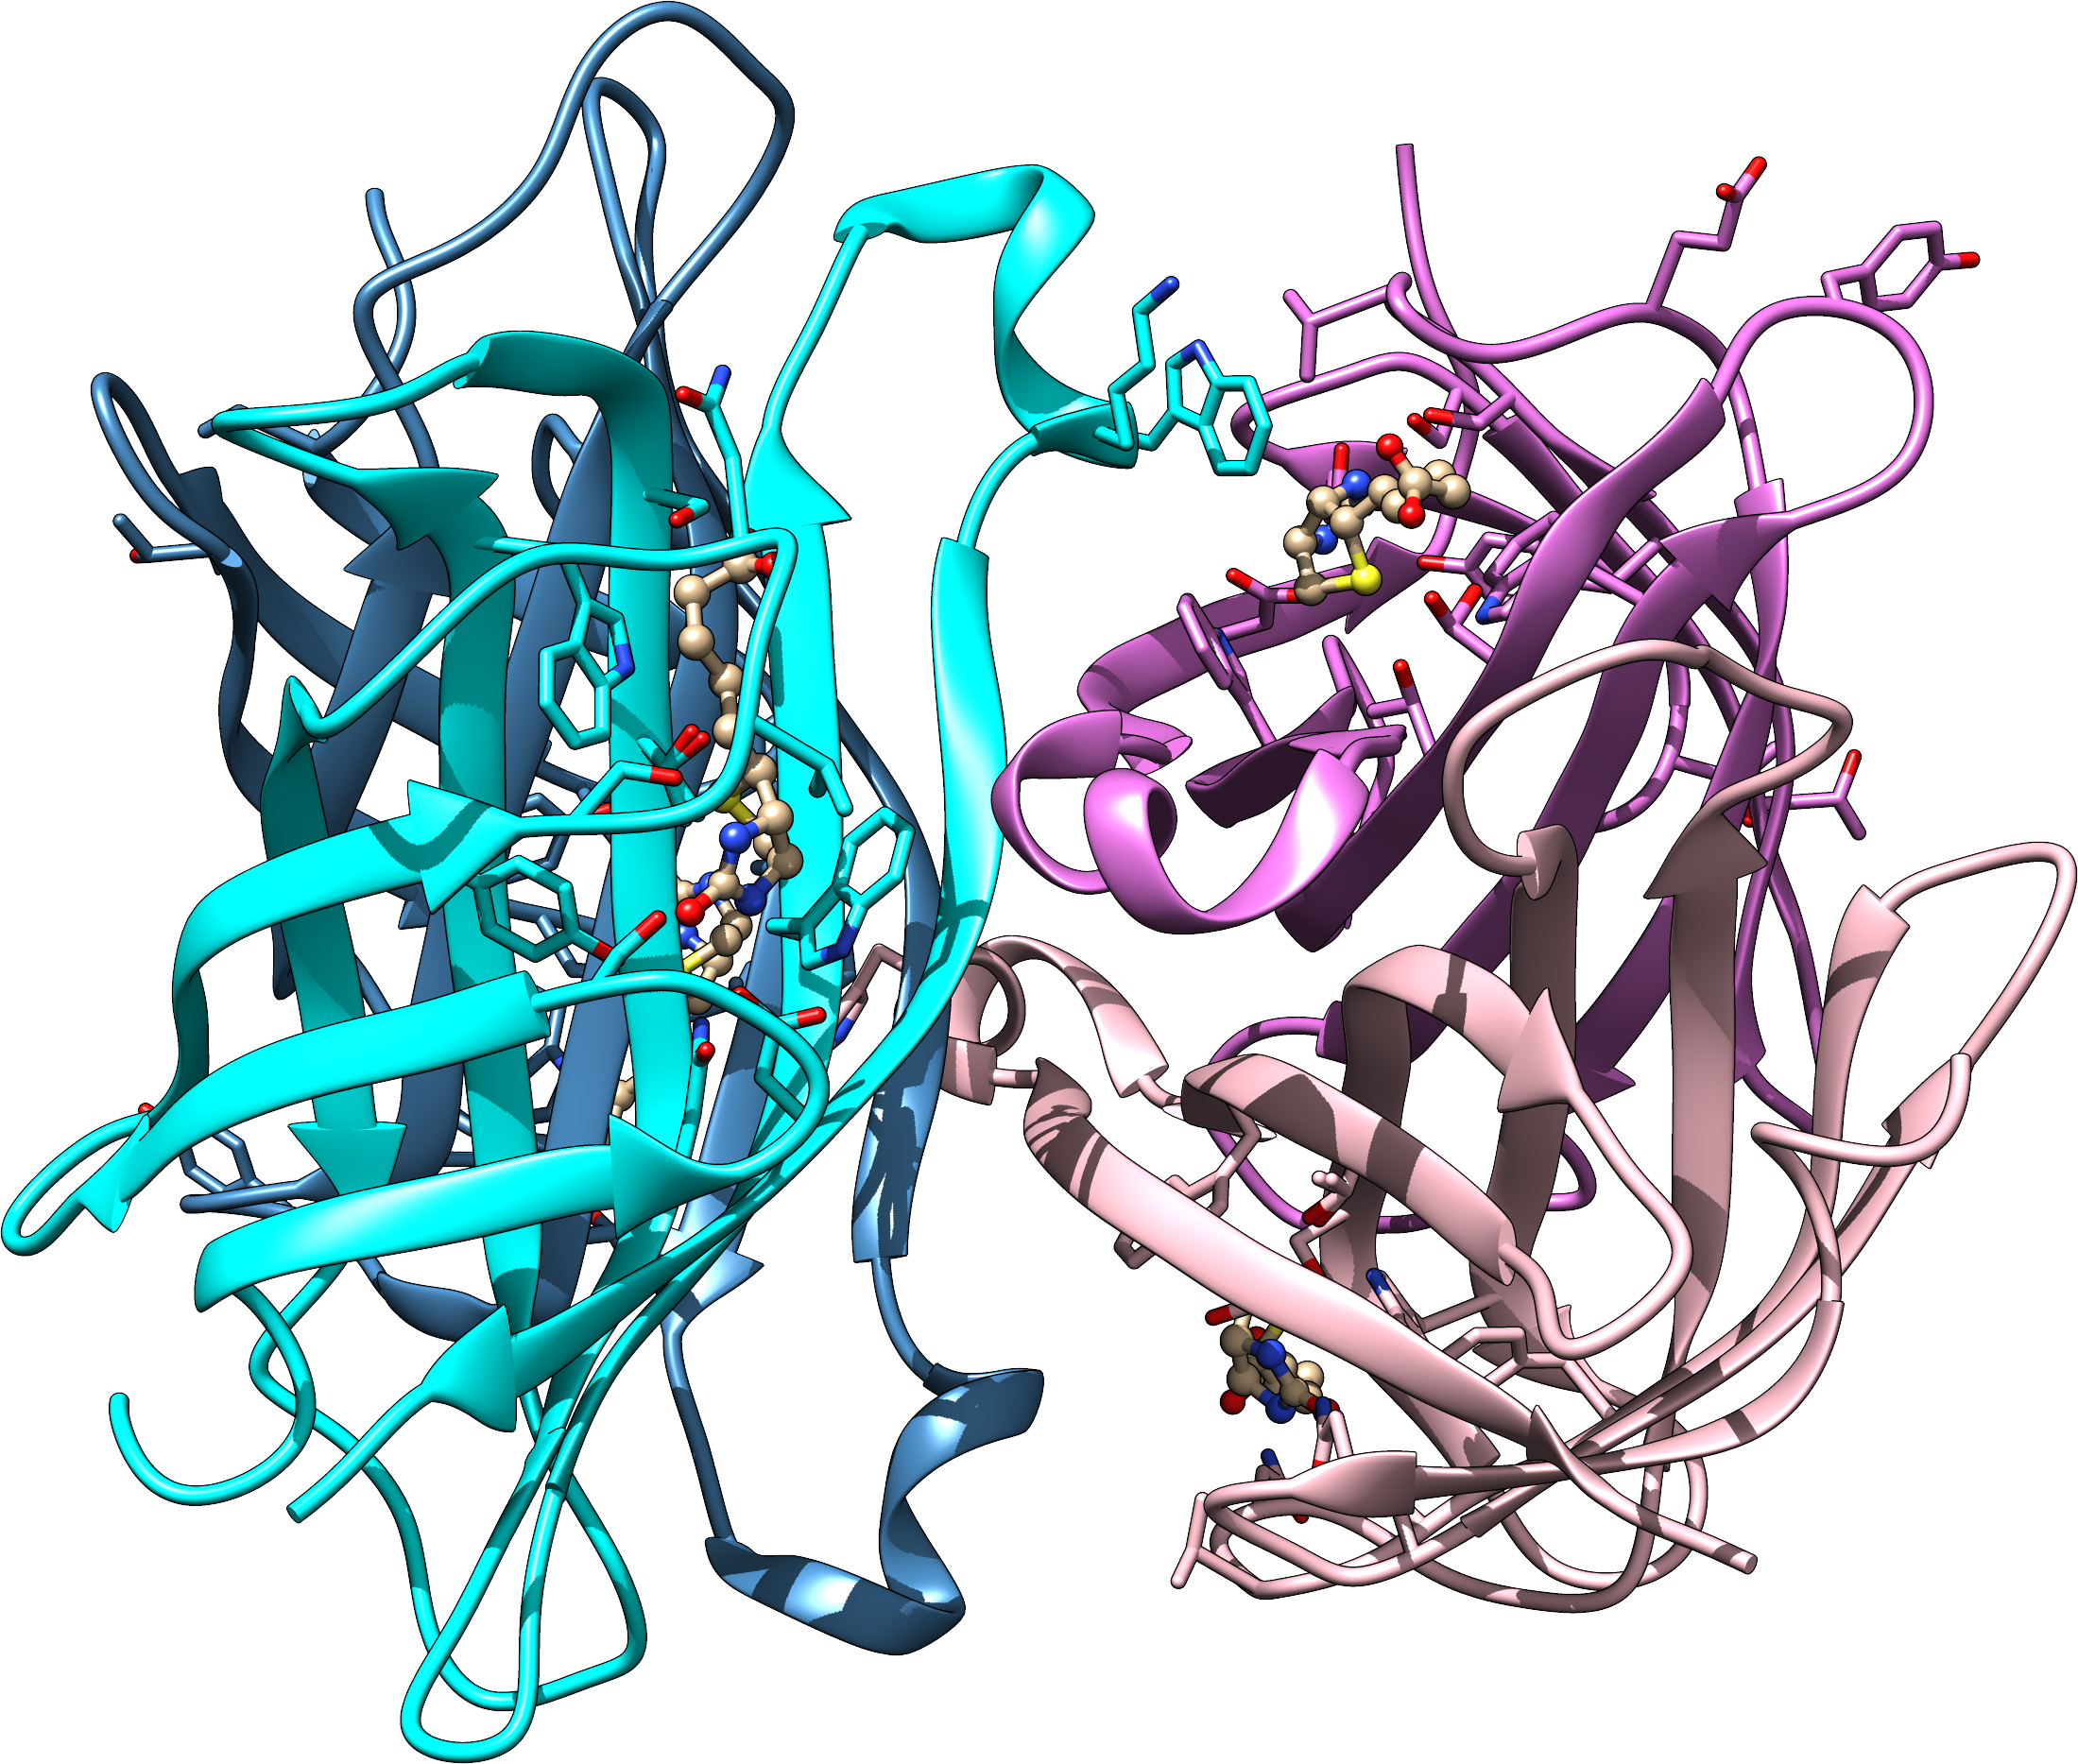
\includegraphics[width=\textwidth]{./figures/06/streptavidin.png}
	\end{Center}
	\caption[Dimer of dimers in streptavidin]{Streptavidin is composed of a dimer of dimers. Each monomer is capable of hosting one biotin molecule. Given its high affinity for biotin, it is a popular system for artificial enzyme design.}
	\label{fig:streptavidin}
\end{figure}

As briefly described in \autoref{chap:04}, the Molecule gene can also be configured to build new molecules by chaining fragments found in a given directory structure. The subdirectories are sorted alphabetically and one fragment is randomly picked from each. The chosen fragments are concatenated following the subdirectory order, using the atoms configured as connectors (first and last atom in the file, by default).



In principle, the dibiotin ligand could be constructed out of five fragments: \textit{biotin A + linker A + cofactor + linker B + biotin B}. However, since biotin exhibits a high affinity for streptavidin, it can be assumed that it will stay in its crystallographic binding site. This allowed to simplify the calculations: instead of having a 5-fragment construction, the biotins were fixed into their crystallographic binding site and a 3-fragment \textit{linker + cofactor + linker} dynamical ligand was used instead (see fig. \ref{fig:dibiotin-linker-length}). To assess if a candidate construct was long-enough to reach both sites, one of the linkers was anchored to one of the biotins following the null-sphere procedure described in \autoref[section]{section:multidocking}. Then, a distance minimization objective was applied to the other linker to push it into the second binding site, where a second biotin was placed to accept the simulated covalent bond. All the bonds in the linkers were allowed to freely rotate with the \texttt{Torsion} gene; biotin and cofactor bonds were considered frozen (see table \ref{table:strep-recipe}).

\begin{table}[hbtp]
	\caption{Recipe applied for the Streptavidin-dibiotin system}
	\label{table:strep-recipe}
	\footnotesize
	\newcolumntype{R}{>{\hsize=.25\hsize\raggedleft\arraybackslash}X}%
	\newcolumntype{L}{>{\hsize=.75\hsize\raggedright\arraybackslash}X}%
	\newcommand{\tableheading}[1]{\multicolumn{2}{c}{\textsc{#1}}}
	\begin{tabularx}{\textwidth}{RL}
		\toprule
		%row no:1
		\tableheading{Genes}\\
		\toprule
		%row no:2
		\texttt{Molecule} & Load the streptavidin dimer, with biotin ligands already frozen in their binding sites  \\
		\midrule
		\texttt{Molecule} & Load a 3-fragment directory to build different versions of the \textit{linkerA-cofactor-linkerB}construction. Linker library included linear alkanes ranging from pentane up to dodecane. The cofactor was DFT-minimized. \\
		\midrule
		\texttt{Torsion} & Explore the flexibility of the linkers (bonds of biotins and cofactor were considered frozen) \\
		\midrule
		\texttt{Search} & Allow free rotation of the ligand from its anchor (end of biotin A), but no translation ($radius=0$) \\
		\toprule
		%row no:4
		\tableheading{Objectives}\\
		\toprule
		%row no:5
		\texttt{Contacts} & Minimize steric clashes between protein and ligand \\
		\midrule
		%row no:6
		\texttt{Angle} & Force an angle of $109.5^\circ$ in anchor point of linker A with biotin A \\
		\midrule
		\texttt{LigScore} & Maximize docking scoring function to select stabilizing interactions \\
		\midrule
		\texttt{Distance} & Minimize the distance between the end of linker B and the end of the biotin B, so the two biotins are connected by the ligand \\
		\bottomrule
	\end{tabularx}
\end{table}

The results showed that a linker compatible with the length of a linear heptane would be enough to reach both binding sites simultaneously. This helped guide the synthesis of the dibiotin ligand (an amide group had to be introduced in the linker, but the suggested length was respected). The resulting ligand exhibits micromolar affinity with streptavidin (manuscript in preparation). Finally, our proposed model also contributed in the refinement process of the X-Ray structure. One of the most interesting parts is that the copper cofactor did not need any type of parameterization for the simulation to work. Simple descriptors like van der Waals overlap can be enough for complex modeling.

\begin{figure}
	\begin{Center}
		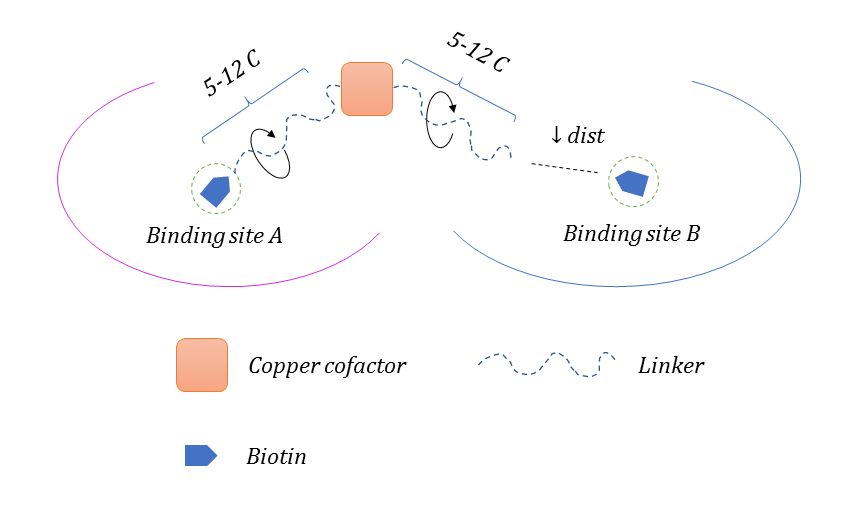
\includegraphics[width=0.9\textwidth]{./figures/06/dibiotin-scheme.png} \\
		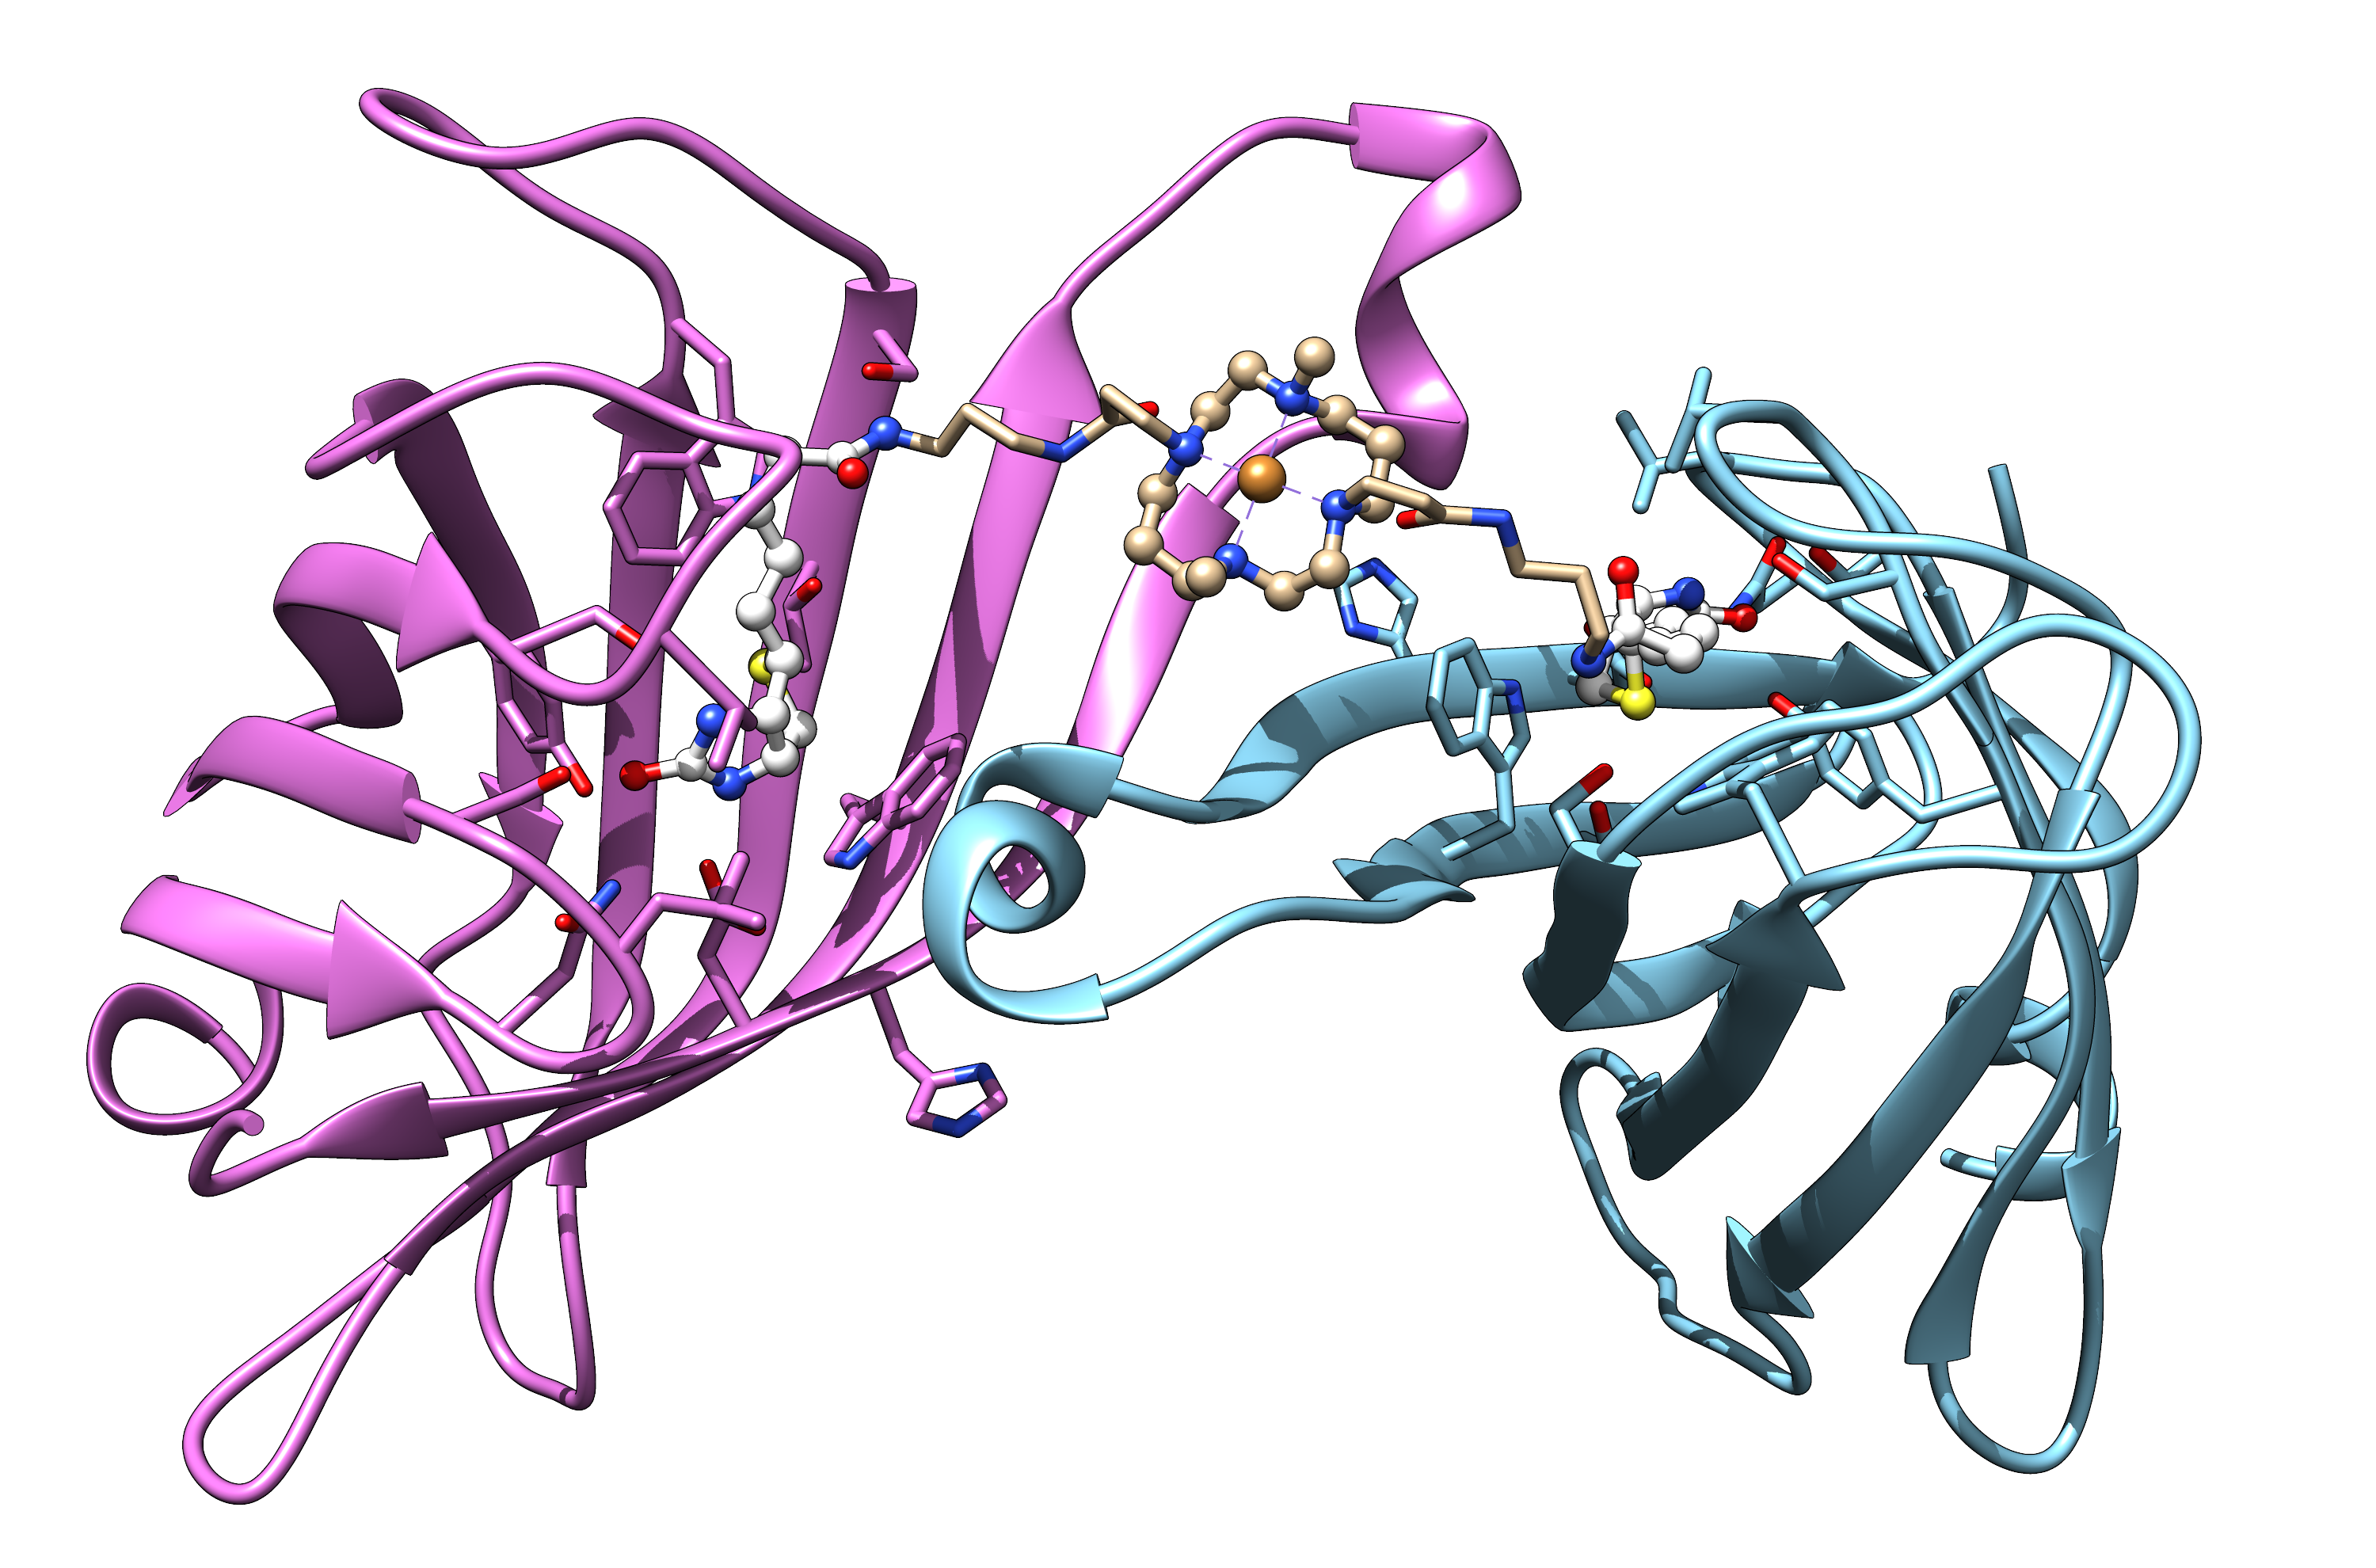
\includegraphics[width=0.9\textwidth]{./figures/06/dibiotin-solution.png}
	\end{Center}
	\caption[Linker length optimization]{To figure out the optimum linker length for  desired dibiotin ligand, a 3-fragment construction was prepared: linker+cofactor+linker. The first linker fragment was anchored to the biotin fixed in binding site A . The copper cofactor and the second linker were appended to its tail. By analyzing the torsions in both the first and second linkers, the end atom in the second linker can reach the biotin already fixed in binding site B. The solution (bottom) proposed a linker compatible with 7-carbon linear alkane.}
	\label{fig:dibiotin-linker-length}
\end{figure}


\subsection{Metal ions: Organization \& binding site prediction}

In two of the previous examples, a metal ion was present in a nonstandard residue. GaudiMM was able to deal with them because the recipes applied did not take any special considerations. All atoms were treated as different-radius spheres connected to other spheres. In some cases, this strategy can be successful, but in others special treatment might be necessary.

This section will present the applications of a novel strategy to deal with metal ions in molecular modeling. Instead of resorting to complex parameterization exercises (see \autoref[appendix]{chap:appendix-c} for further details) like those expected in Molecular Mechanics, some properties of the metal ions can be described with geometry measurements.

\subsubsection{Restrained conformational analysis for Alzheimer's β-amyloid peptide}

Conformational analysis can be described as a range of techniques focused on taking an input molecular structure and generating coordinates sets (conformers) compatible with a set of criteria, normally energetic and geometric. This definition is broad enough to be used for other type of studies, such as the aforementioned docking variants, but is also a direct reflection on how GaudiMM impose a clear separation of concerns when it comes to exploration and evaluation. Once again, generating those new coordinate sets is a matter of choosing the right \textit{genes}, and deciding if they are compatible with some criteria or not is up to the \textit{objectives}.

To perform conformational analysis only one operation is needed: modify the coordinates set sensibly. This can be performed in a high-temperature molecular dynamics simulation, but parameters would be needed beforehand. For simple cases, GaudiMM's Torsion gene can be employed: all bonds lengths will be restrained to those in the input structure, but dihedral exploration will be performed on those bonds considered rotatable. Using the Contacts objective can help minimize the steric clashes and additional constraints like distances and angles can be imposed so the proposed solutions are compatible with a given geometry. The resulting calculation could be regarded as a restrained conformational analysis, very useful for finding initial structures of unparametrized small molecules you want to study with higher levels of theory, such as QM.

For some peptides, the same \texttt{Torsion} applied in small molecules can be applied to test the torsion angles of the CO--NH peptide bonds. This would result in the exploration of the backbone flexibility. This idea can be coupled with the \texttt{Rotamers} gene to assess the conformational variability of the sidechains. For the evaluation, full MM energy can be calculated with the \texttt{Energy} objective. Additional restraints are supported via the corresponding objectives: \texttt{Angle} and \texttt{Distance} for geometrics, and \texttt{Surface} and \texttt{Volume} for volumetrics.

In the GaudiMM manuscript, an unbound Alzheimer's β-amyloid structure was processed following this strategy in an attempt to reproduce experimental Zn-bounded NMR models (PDB ID 1ZE9\cite{pdb:1ze9}).

Starting with the unfolded peptide (PDB ID 1ZE7\cite{pdb:1ze7}), its backbone torsions were analyzed in hope of findind a combination of rotations that could be compatible with those in the Zn-bounded form. The only evaluators used were: (1) a Contacts minimization to rapidly discard structures with abundant steric clashes, (2) an Energy minimization with the Amber 99 SBILDN force field for more accurate values, and (3) a Volume objective configured to match the average volume occupied by the 20 Zn-bound NMR structures reported in PDB ID 1ZE9 (15854 Å\textsuperscript{3}), intrinsically showing a possible pre-organization of the isolated peptide. Even though the Zn ion was not explicitly considered, proposed structures were in agreement with the experimental ones, with backbone RMS deviations in the range of 3.5 \AA (see fig. \ref{fig:peptide-folding}).


\begin{figure}
	\begin{Center}
		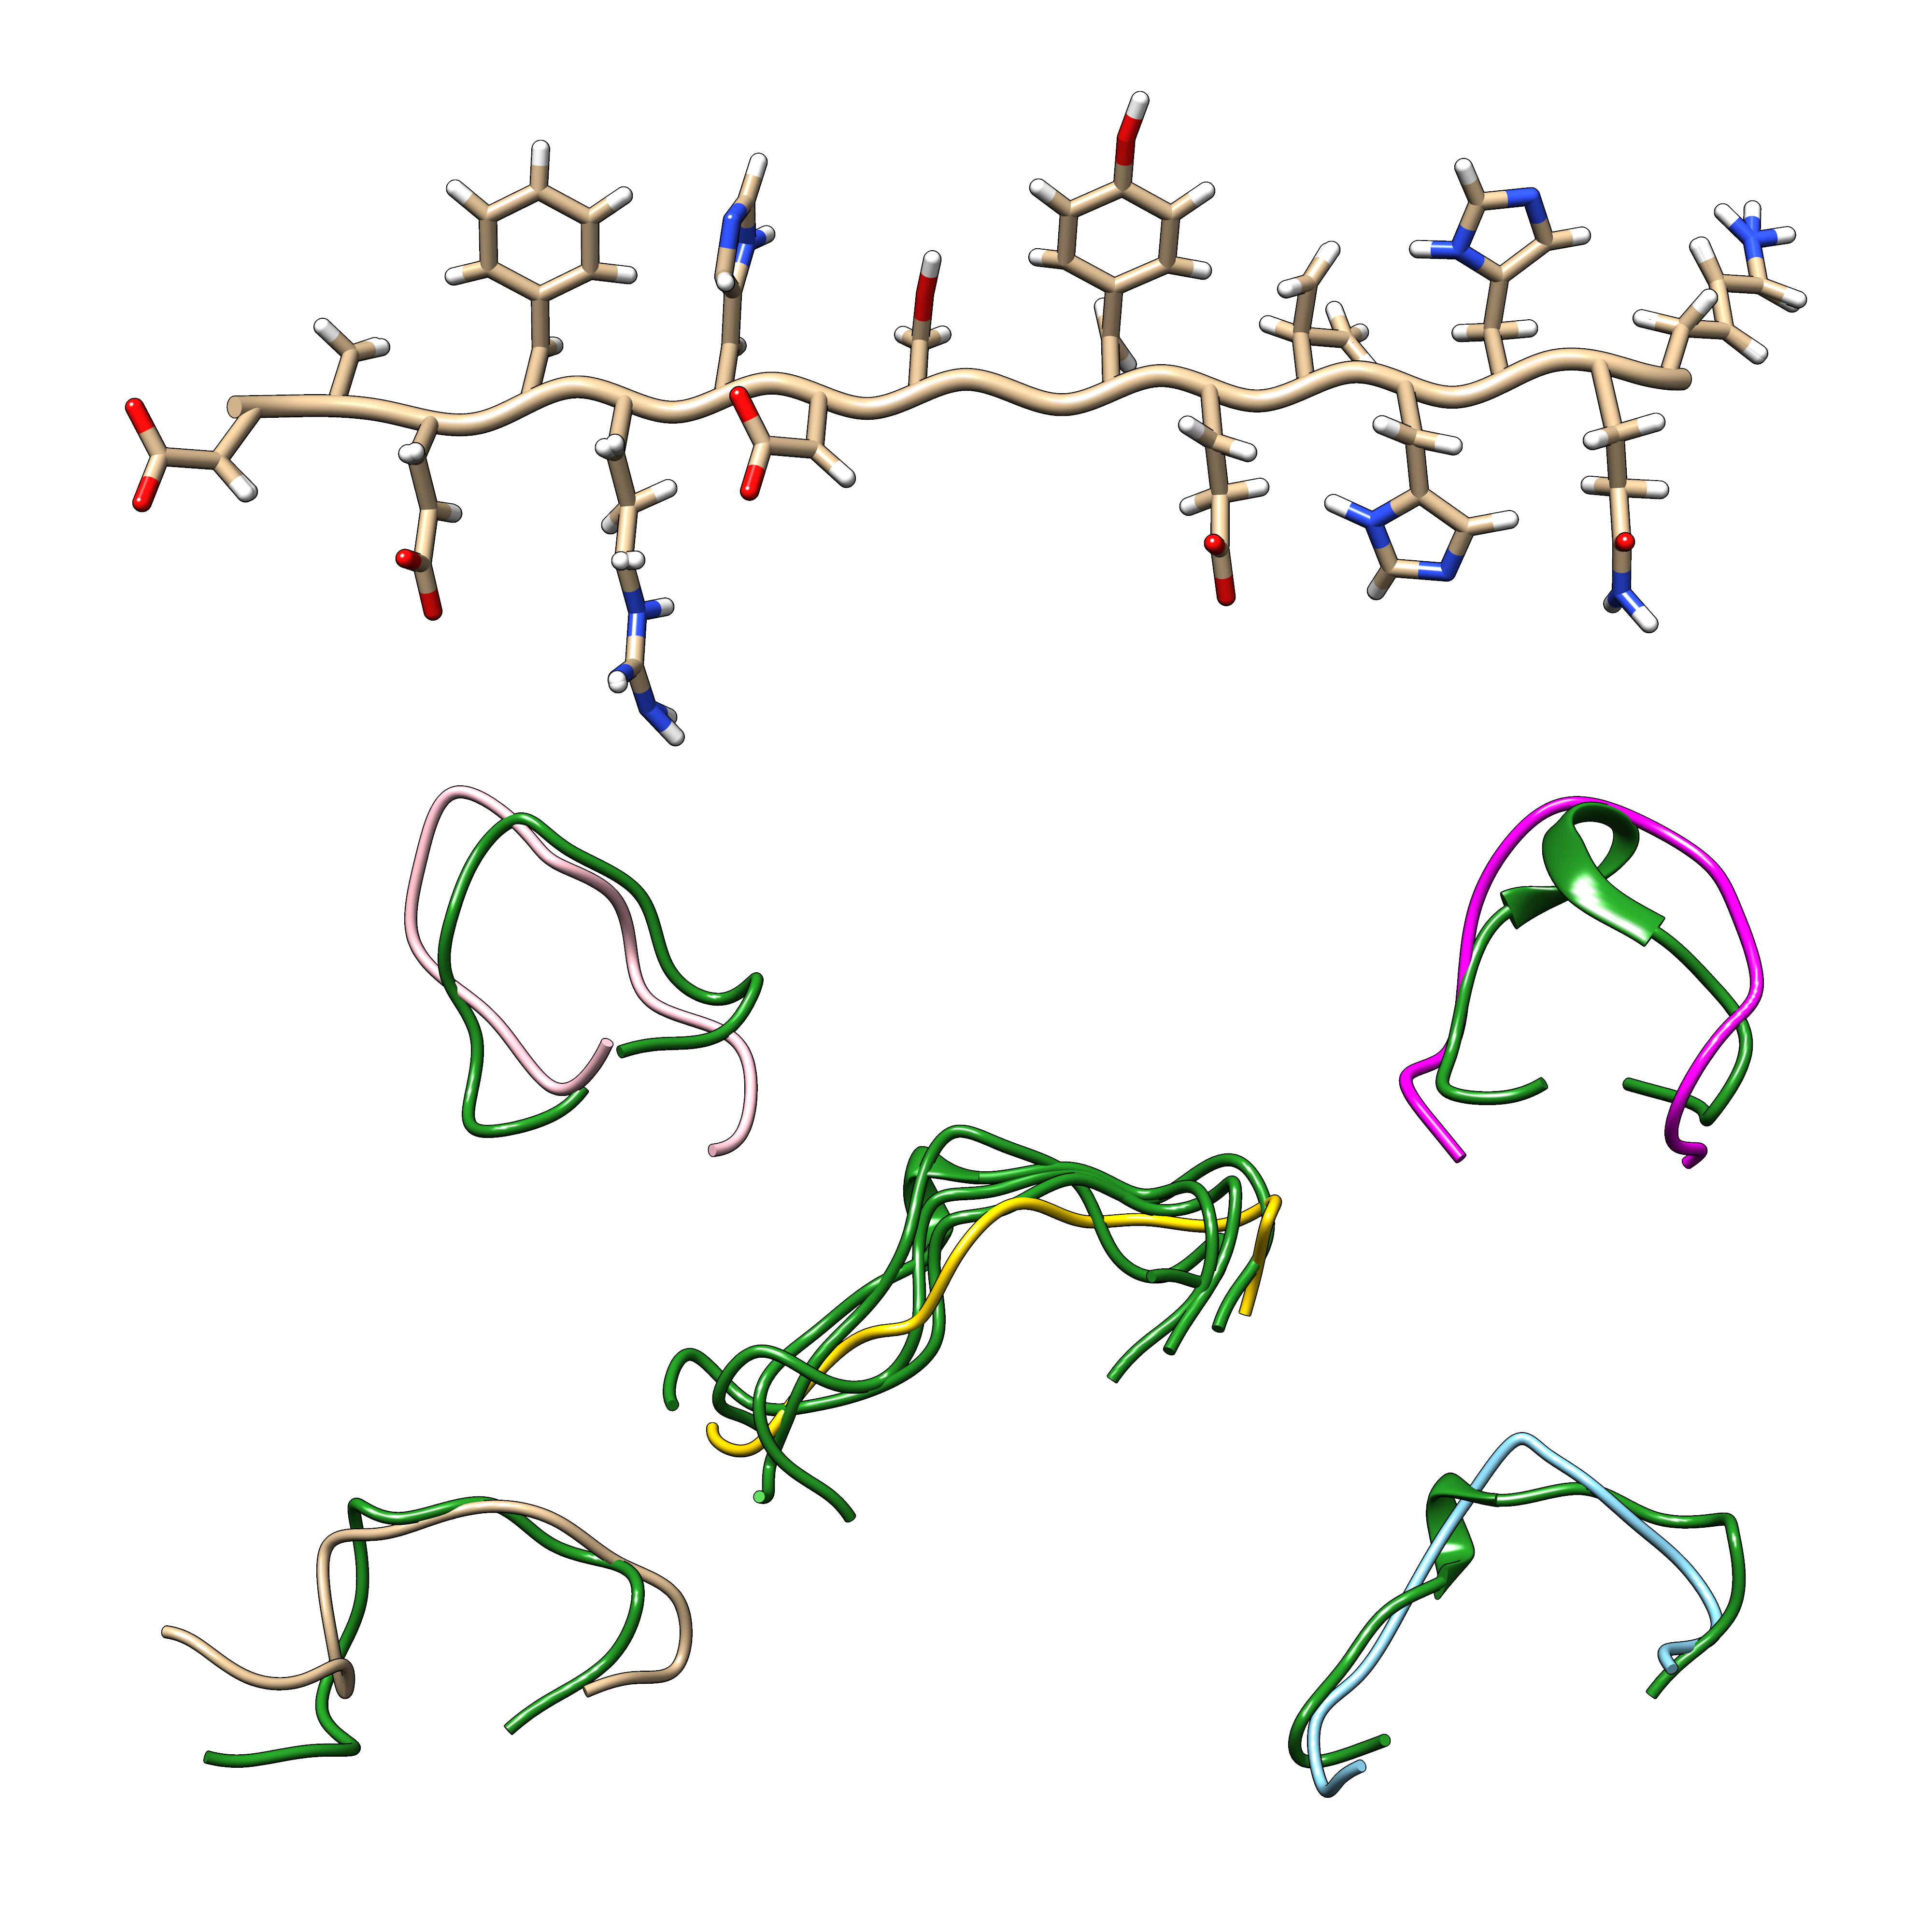
\includegraphics[width=\textwidth]{./figures/06/peptide-folding.png}
	\end{Center}
	\caption[Peptide folding]{Unfolded peptides can adopt feasible folded structures under a given volume only by exploring backbone torsion angles and force field energy minimization objectives. Low-energy solutions were further aligned to their best NMR conformation matches (in green).}
	\label{fig:peptide-folding}
\end{figure}


\subsubsection{Finding metal binding sites in biomolecules}
% \addcontentsline{toc}{subsection}{Metal-centric docking: coordination-guided explorations}

Metal-protein and metal-peptide interactions are not unusual at all: around 30\% of the human genome encodes for metal-containing biomolecules.\cite{rehder2014bioinorganic} As a result, having the ability to describe and predict these interactions becomes an interesting exercise in molecular modeling.

GaudiMM features an objective specifically designed for that purpose: the \texttt{Coordination} objective. The idea  was initially described in Mujika et al,\cite{mujika2017elucidating} where a multi-objective docking procedure was used to locate possible octahedral coordination sites of an aluminum ion within pre-optimized structures of Alzheimer's β-peptides. The octahedral geometry could be described by using several distances, angles and dihedral objectives\footnote{This was done with a very early version of GaudiMM, when the notion of objective was in development. As a result, some of the modules here listed do not have an exact correspondence with the current ones.} set to match those in an ideal octahedron: coordination bonds of around 2 \AA, $90^{\circ}$  for the donor-metal-donor angle, and a dihedral of $109.5^{\circ}$  for compatible sp\textsuperscript{3} geometries (see table \ref{table:alum-recipe}).

\begin{table}[hbtp]
	\cprotect\caption{Recipe applied for the Al(III)-amyloid complexes.}
	\label{table:alum-recipe}
	\footnotesize
	\newcolumntype{R}{>{\hsize=.25\hsize\raggedleft\arraybackslash}X}%
	\newcolumntype{L}{>{\hsize=.75\hsize\raggedright\arraybackslash}X}%
	\newcommand{\tableheading}[1]{\multicolumn{2}{c}{\textsc{#1}}}
	\begin{tabularx}{\textwidth}{RL}
		\toprule
		%row no:1
		\tableheading{Genes}\\
		\toprule
		%row no:2
		\texttt{Molecule} & Load the preoptimized peptide, without the aluminium  \\
		\midrule
		\texttt{Molecule} & Load the bare aluminium ion \\
		\midrule
		\texttt{Search} & Allow free translation of the aluminium ion within 5 \AA \\
		\toprule
		%row no:4
		\tableheading{Objectives}\\
		\toprule
		%row no:5
		%row no:6
		\texttt{Contacts} & Minimize steric clashes (stops the aluminium from getting too close) \\
		\midrule
		\texttt{Distance} (x3) & Optimize the distance from the aluminium ion to the (three) closest oxygen atoms \\
		\midrule
		\texttt{Dihedral} (x3) & Align the dihedral angles between the coordinating residues and the aluminium position \\
		\bottomrule
	\end{tabularx}
\end{table}


After validating the utility of this proof-of-concept, a first generalization of the method was implemented as a separate objective in GaudiMM, and tested in some illustrative cases for its publication (see \autoref[section]{section:siderophore}).

In short, the \texttt{Coordination} objective scans the surroundings of the selected metal ion for suitable donor atom types (like terminal sp\textsubscript{3} oxygen atoms in aspartic acid). If sufficient donors are found within 3.0 \AA, their positions with respect to the metal center are compared to those of the vertices of the corresponding ideal polyhedron. This comparison is performed with a point-set registration method called Coherent Point Drift,\cite{myronenko2010point} which admits missing points. This means that geometries with vacant vertices can be considered seamlessly. If the comparison is successful, a RMSD value is returned and two additional checks are calculated: (1) the directionality of the hypothetical coordination bond is assessed through the absolute difference of the sines of the angles and dihedrals of the involved atoms against the ideal ones, and (2) the ideal distance is compared to the measured distance and the absolute difference is. All these terms are summed linearly, which should result in a value of zero for perfect geometries. By minimizing this function over a few generations, coordination geometries can be identified.

\begin{figure}[H] % FIXME!
	\begin{Center}
		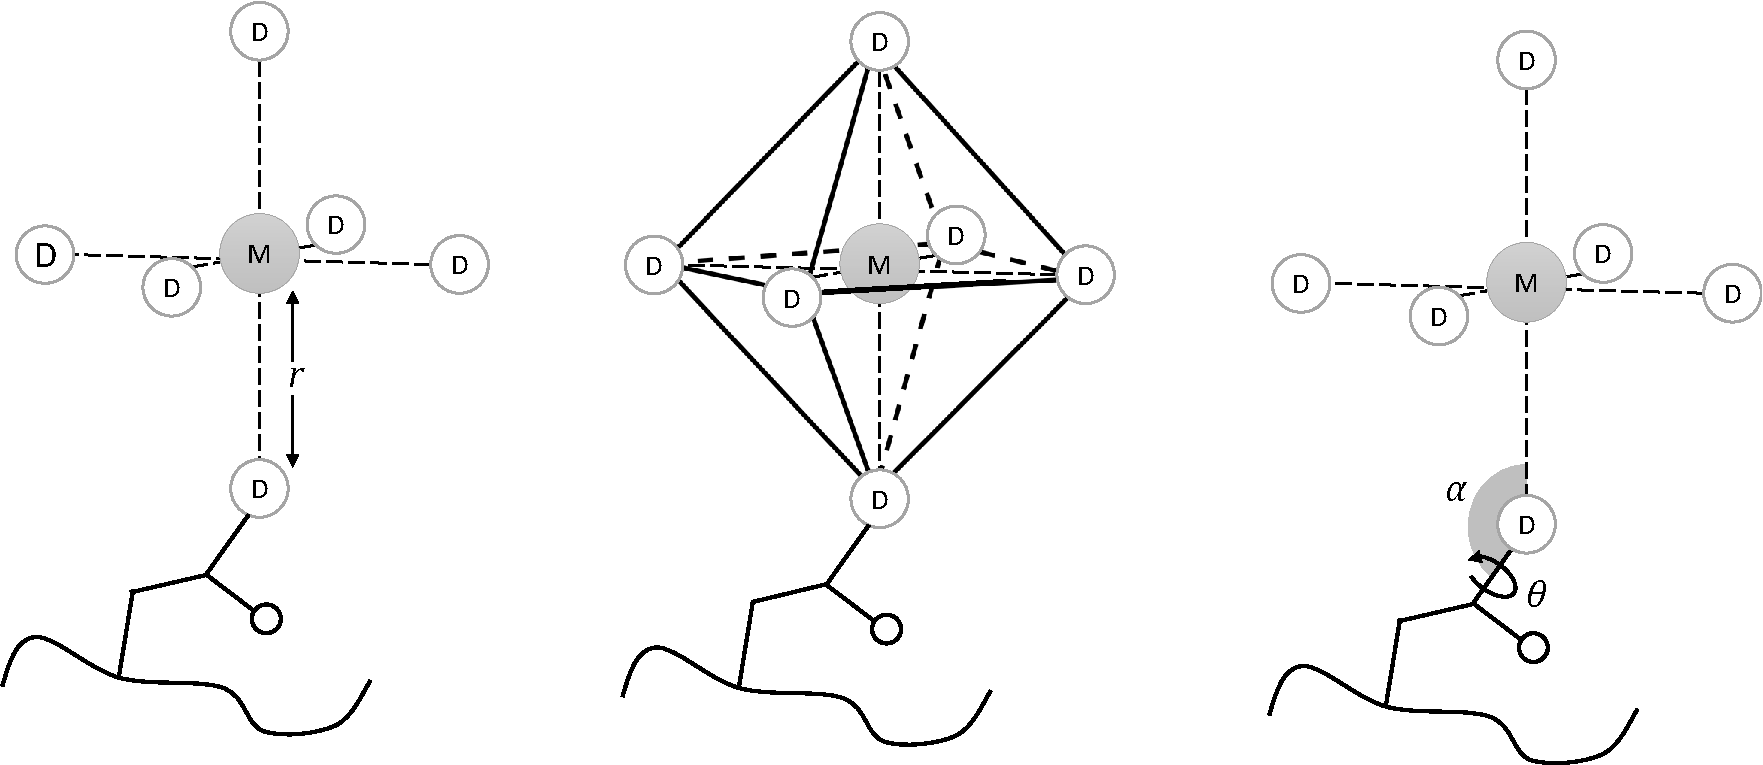
\includegraphics[width=\textwidth]{./figures/06/coordination-crop.pdf}
	\end{Center}
	\cprotect\caption[Coordination objective]{In the \texttt{Coordination} objective, a metal ion $M$ queries its surroundings looking for potencial coordinating atoms (donors, $D$). If the number of donors is enough, a Coherent Point Drift registration is performed to match the ideal polyhedron and the directionalities of the bonds are checked.}
	\label{fig:coordination-objective}
\end{figure}


A posterior refinement of this objective has been extensively reviewed recently,\cite{gaudimetals} where we discuss different modifications of the initial score function. The most promising is benchmarked against a dataset of 106 high-quality X-ray metal-containing proteins representing diverse metallic species with octahedron-derived geometries. The protocol considers a 20 Å radius for the search sphere and a rigid protein structure. With these updates, the initial success rate increased from an initial 86$\%$  to a final 100$\%$. If flexibility of sidechains is considered with the \texttt{Rotamers} gene, the success rate retains a value of 87.5 $\%$, even with the added search dimensionality.

\subsubsection{Folding metal-bound siderophores}
\label{section:siderophore}

Siderophores are key compounds in the metabolic access to iron species, involved in oxygen transport and other vital processes. Since Fe\textsuperscript{3+} has bad solubility in water, these are responsible for their chelation and intake. Enterobactin is the strongest siderophore known ($K = 10^{52} M^{-1}$) and is primarily found in Gram-negative bacteria. An iron-free 3D structure can be found in PubChem,\cite{Enterobactin} which substantially differs from its metal-bound form found in bacterial proteins, like \textit{E. coli}'s FepB.\cite{3tlk}

To assess the guiding capacities of the \texttt{Coordination} objective, an illustrative case was proposed in GaudiMM's original publication. The task was to fold the iron-free form into its metal-bound form. A \texttt{Torsion} gene was configured to explore rotatable bonds of the unfolded siderophore structure, and a \texttt{Search} gene was instructed to move the iron ion within a radius of 5 \AA.

The main driver of the optimization was the Coordination objective, which was set up to find octahedral geometries by analyzing terminal oxygen atoms. This strategy successfully reproduced three of the four structures found in \textit{E. coli}'s FepB. RMSD values were under 1.0 Å in all cases (see table \ref{table:siderophore} and fig. \ref{fig:siderophore}).

\begin{table}[hbtp]
	\caption{Recipe applied for the enterobactin exercise}
	\label{table:siderophore}
	\footnotesize
	\newcolumntype{R}{>{\hsize=.25\hsize\raggedleft\arraybackslash}X}%
	\newcolumntype{L}{>{\hsize=.75\hsize\raggedright\arraybackslash}X}%
	\newcommand{\tableheading}[1]{\multicolumn{2}{c}{\textsc{#1}}}
	\begin{tabularx}{\textwidth}{RL}
		\toprule
		%row no:1
		\tableheading{Genes}\\
		\toprule
		%row no:2
		\texttt{Molecule} & Load the unfolded enterobactin\cite{Enterobactin} \\
		\midrule
		\texttt{Molecule} & Load a bare iron ion \\
		\midrule
		\texttt{Torsion} & Explore the flexibility of the rotatable bonds in enterobactin \\
		\midrule
		\texttt{Search} & Move the iron within 2.5 \AA \\
		\toprule
		%row no:4
		\tableheading{Objectives}\\
		\toprule
		%row no:5
		\texttt{Contacts} & Minimize steric clashes in the system \\
		\midrule
		%row no:6
		\texttt{Coordination} & Match an octahedral geometry by querying the terminal oxygen atoms of the enterobactin rings \\
		\midrule
		%row no:6
		\texttt{Distance} & Since UCSF Chimera does not support dihedral torsions in closed rings, the central ring of the enterobactin was deliberately opened so their torsion bonds could be explored. This distance keeps the ring functionally closed while that happens. \\
		\bottomrule
	\end{tabularx}
\end{table}


\begin{figure}[H] % FIXME!
	\begin{Center}
		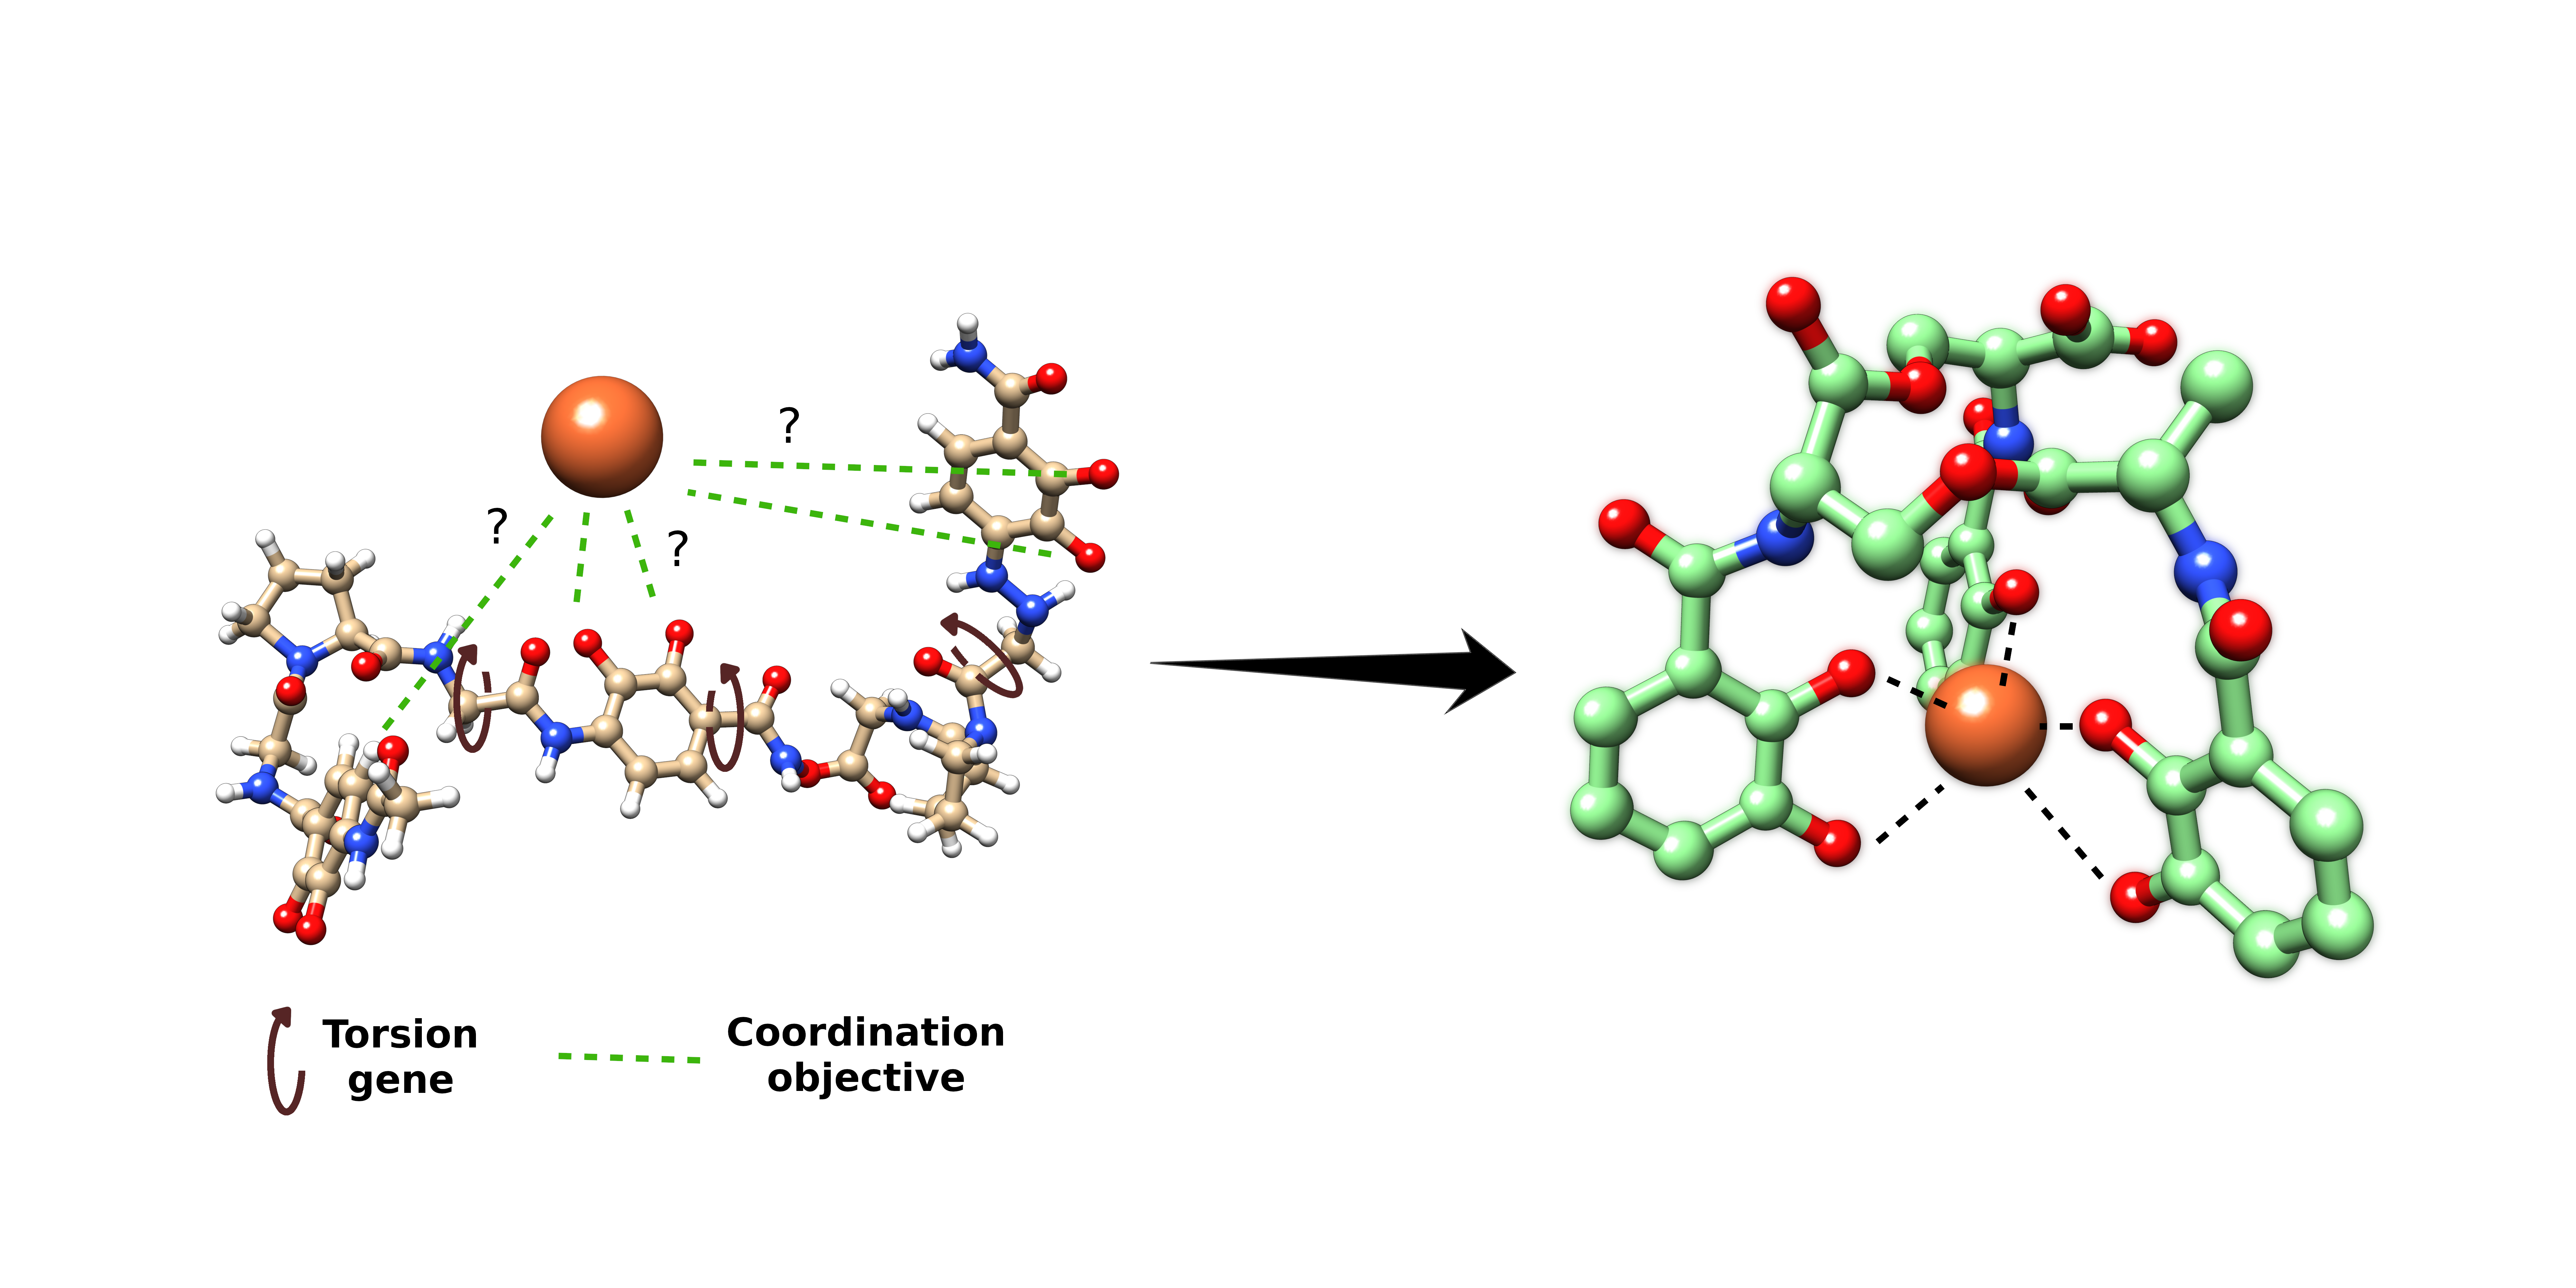
\includegraphics[width=\textwidth]{./figures/06/siderophore.png}
	\end{Center}
	\cprotect\caption[Siderophore folding]{GaudiMM can transform an unfolded apo-enterobactin siderophore into its metal-bound form as found in \textit{E. coli} FepB by exploring its free-torsion bonds to find an octahedral coordination geometry around an iron ion.}
	\label{fig:siderophore}
\end{figure}


%%%%%%%%%%%%%%%%%%%%%%%%%%%%%%%%% SECTION 2 %%%%%%%%%%%%%%%%%%%%%%%%%%%%%%%%%%%%%

\section{Case study: Multiscale modeling of multivalent enzyme inhibitors}
% \addcontentsline{toc}{section}{Multiscale modeling of multivalent enzyme inhibitors}
GaudiMM was conceived to be the entry door to the multiscale funnel, while the tools presented in \autoref{chap:05} fill in other gaps down the funnel. In this section, a real example on how all these developments work together and allow to create integrative workflows is presented. It is a deep computational insight on the work described in \textit{Pillar[5]arene glyco(mimetic)rotaxanes for the functional interrogation of multivalency responsive glycosidases},\cite{rotaxane} a collaboration with the IIQ-CSIC in Seville, Spain.

\subsection{Introduction to multivalent enzyme inhibition}
% \addcontentsline{toc}{subsection}{Introduction to the problem}
Biological molecules are usually classified in four separate families: nucleic acids, lipids, saccharides and proteins. Far from being separate entities, they can be found together in many processes. A particularly interesting combination is when proteins and saccharides work together.

A protein featuring covalently attached oligosaccharidic chains (or glycans) is called a glycoprotein. Glycoproteins are key recognition processes such as those in the mammal immune system, but can also be used for like solvent retention in extracellular secretions that demand high viscosity (mucus) or protection against freezing damage.

However, not all protein-saccharidic collaborations are strictly covalent. Glycoside hydrolases (or glycosidases) can specifically recognize glycosides and\ catalyze the hydrolysis of their intermonomer bonds in complex sugars.  They are key in natural polymers degradation like starch (amylase) or cellulose (cellulase), pathogenesis, anti-bacterial activity (lysozyme) and normal cell function. Other examples are lectins, which exhibit high affinity for specific saccharidic residues through non-bonded interactions. They are involved in biofilm formation,\cite{tielker2005pseudomonas} immune response\cite{turner1996mannose} or even antineoplastic activities,\cite{adwan2014} to name a few. Studying mechanisms of inhibition would allow to develop new antibacterial techniques or avoid biofilm formation, for example.

Most common strategies for enzyme inhibition involve designing a mimetic ligand that can block the binding site of the substrate through a key-and-lock mechanism preventing the enzyme from performing any further action. For lectins and glycosidases, glycomimetic compounds like iminosugar-containing ligands can be employed. Iminosugar moieties are standard saccharides whose oxygen atom in the ring has been replaced by a nitrogen atom. The first iminosugar characterized, 1-deoxynojirimycin (DNJ) was isolated from a natural source and showed to be an alpha-glucosidase inhibitor with anti-diabetic and antiviral activities. Since then, more iminosugars have been described in the literature.

Recently, the general intuition around the classical lock-and-key inhibition behavior was recently questioned in a study that described 2000-fold inhibition enhancement towards the Jack bean $\beta$-mannosidase (JbM) when twelve copies of DNJ were displayed around a $C_{60}$ fullerene.\cite{compain2010glycosidase} The strategy, termed Multivalent Enzyme Inhibition (MEI), was then observed in other systems. Knowing that JbM has a very accessible binding pocket and is multimeric in solution provides an understandable rationale behind this enhancement: a single C60 construct can block several sites at once. However, this idea cannot explain why monomeric enzymes with deep and narrow binding pockets are also inhibited by bulky multivalent conjugates. Additionally, it has been observed that putative sugars also inhibit their corresponding catalytic enzymes if they are multivalently displayed in a conjugate, defying the assumption of specificity and non-promiscuity glucosidases are thought to exhibit.

\subsection{Experimental results}

To shed light on such counterintuitive phenomena, García-Fernández \textit{et al }specifically designed a series of two-component pillar[5]arene rotaxane conjugates that exhibited both glycomimetic and non-glycomimetic (putative) residues. The first component is a H-shaped central axel, which exhibits four sp\textsuperscript{2}-iminosugar-type\textsuperscript{[12]} 6-oxa-5\textit{N},6\textit{O}-oxomethylidenenojirimycin (ONJ) residues, one on each on the stop caps. The second component is the pillar[5]arene, which exhibits ten moieties of glucose, mannose or galactose, depending on the variant, one on each of its ten rims (see fig. \ref{fig:rotaxane-compounds}).

To test the contribution of the multivalent saccharides, two reduced models that did not account for the pillar[5]ene were also considered: 1) a monovalent ONJ compound only bearing the hexyltriazolyl aglycone segment present in the rotaxane, and 2) a divalent ONJ compound, which emulates one of the stoppers halves of the central axel of the rotaxane.



\begin{figure}[H] % FIXME!
	\begin{Center}
		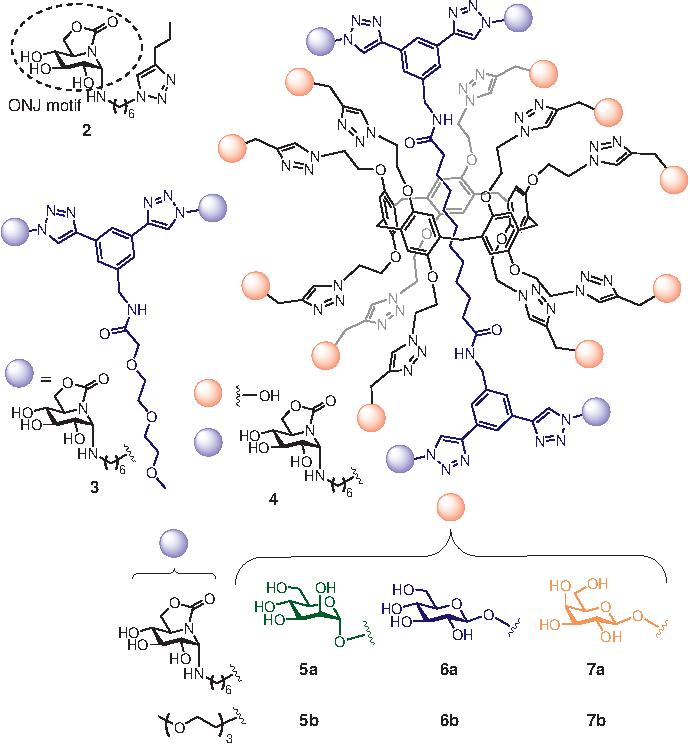
\includegraphics[width=\textwidth]{./figures/06/glyco-inhibitors-crop.pdf}
	\end{Center}
	\cprotect\caption[Tested inhibitors against ScGH13 and TmGH1]{Different inhibitors variants tested against the monomeric ScGH13 and dimeric TmGH1 proteins. In the computational studies, only divalent model (number 3) and rotaxane variant 5a were tested. Reproduced from Nierengarten, 2018.\cite{rotaxane}}
	\label{fig:rotaxane-compounds}
\end{figure}



All these inhibitors and their controls were tested and measured on two glycosidases for which crystallographic data evidenced the existence of deep binding pockets: the monomeric GH13 α-glucosidase from \textit{Saccharomyces cerevisiae} (\textit{ScGH13}, yeast maltase) and the dimeric GH13glucosidase from \textit{Thermotoga maritima} (\textit{TmGH1}). The inhibition potency was measured experimentally and reported in $ \mu M $ units (see table \ref{table:glycosidase-inhibition}). Further details are out of the scope of this dissertation but can be found in the manuscript.


%%%%%%%%%%%%%%%%%%%% Table No: 2 starts here %%%%%%%%%%%%%%%%%%%%


\begin{table}[H]
	\cprotect\caption[Glycosidases inhibition tests]{ $K_{i}$ (in $ μM $) for the different inhibitors tested against the monomeric ScGH13 and dimeric TmGH1 proteins. Reproduced from Nierengarten, 2018.\cite{rotaxane}}
	\label{table:glycosidase-inhibition}
	\footnotesize
	\newcolumntype{C}{>{\centering\arraybackslash}X}%
	\begin{tabularx}{\textwidth}{CCCCCCC}
		\toprule
		\multirow{2}{*}{$K_{i}~^{a}$} & \multicolumn{2}{c}{ONJ} & \multicolumn{4}{c}{Pillar-[5]-arene} \\   \cmidrule(l){2-3} \cmidrule(l){4-7}
								&	Monovalent & Divalent & Regular & \textsc{d}-\textit{manno} & \textsc{d}-\textit{gluco} & \textsc{d}-\textit{galacto} \\ \midrule
		%row no:2
		ScGH13\textsuperscript{b} &
		$ 4.3 \pm  0.5 $ &
		$ 2.5 \pm  0.3 $ &
		$ 2.3 \pm  0.1 $ &
		$ 33 \pm  2 $ &
		$ 16 \pm  1 $ &
		$ 13 \pm  1 $ \\
		\midrule
		%row no:3
		TmGH1\textsuperscript{c} &
		$ 109 \pm  5 $ &
		$ 3.0 \pm  0.2 $ &
		$ 7.1 \pm  0.3 $ &
		$ 6.3 \pm  0.3 $ &
		$ 16 \pm  2 $ &
		$ 27 \pm  2 $ \\
		\bottomrule
		\multicolumn{7}{p{0.9\textwidth}}{\textit{\textsuperscript{a}Measured in $\mu M$. \textsuperscript{b}Monomeric. \textsuperscript{c}Dimeric}} \\

	\end{tabularx}
\end{table}


%%%%%%%%%%%%%%%%%%%% Table No: 2 ends here %%%%%%%%%%%%%%%%%%%%



For the monomeric ScGH13, results were not surprising: the monovalent ONJ is a strong inhibitor with $K_{i} = 4.3 \pm 0.5 \mu M $, and the divalent ONJ shows a 1.7-fold enhancement explainable by statistics alone: two iminosugar moieties are available in each molecule. The pillar[5]ene variant, featuring four iminosugars, should have increased that value again but stayed at $ 2.3 \pm 0.1 \mu M $ . The trend was not the same in the dimeric TmGH1, though. The monovalent ONJ model was a very weak inhibitor ($ K_{i} = 109 \pm 5 \mu M$), but the divalent variant showed a 36-fold enhancement ($ K_{i} = 3.0 \pm 0.2 \mu M$). The pillar[5]ene variants did not improve this Ki but did not cancel it either.

This surprising enhancement in the inhibition power of the divalent ONJ compound towards the dimeric TmGH1 could not be explained by stoichiometry alone. One hypothesis was to consider that the dimeric conformation observed in the X-Ray data was not the only one present in solution, leaving room to the idea that the divalent ONJ compound was able to reach the binding sites of two hypothetical monomers at the same time and force a blocked dimerization. However, for that to be possible the di-ONJ ligand must be long enough, something that was not entirely safe to assure. If a single di-ONJ ligand was not enough, could two di-ONJ molecules occupy a binding site each and then stabilize each other via the free ONJ end? What about the hydrophobic tail? Is the same interaction profile feasible for the pillar[5]arene variants? At this point, computational insights were requested in hopes of finding structural models that could help explain the experimental observations. The questions posed are summarized now:

\begin{itemize}
	\item Can a single di-ONJ ligand reach both sites? If not, how long should it be?
	\item Can two di-ONJ ligands occupy both sites simultaneously? Do they interact?
	\item Does the pillar-[5]-ene compound fit in the dimer? Can it occupy both sites comfortably? If so, in which conformation?
\end{itemize}

\subsection{Computational approaches towards an explanation}
% \addcontentsline{toc}{subsection}{Methods $\&$  results}
A project like this, in which computational insights are needed to clarify experimental observations, is perfect to prove how GaudiMM allows to formulate (bio)chemical hypothesis as optimization problems solvable by a multi-objective genetic algorithm. Each question might need a slightly different resolution strategy, which will be described in the following subsections, but the main protocol remains the same:

\begin{enumerate}
	\item The problem is formulated as a combination of genes and objectives in GaudiMM.

	\item All the candidate structures are analyzed interactively with GaudiView and any needed Tangram extensions. Interaction profilers are particularly useful at this stage.

	\item Best-looking candidates are checked for stability with long molecular dynamics trajectories (more than 100 ns). The protocol involves using explicit solvent and full-atom treatment using the GPU acceleration provided by OMMProtocol.
\end{enumerate}

\subsubsection{Can a single divalent ligand reach both sites? If not, how long should it be?}
% \addcontentsline{toc}{subsubsection}{Can a single divalent ligand reach both sites? If not, how long should it be?}
\label{section:di-ONJ-stretch}
The Ki of the divalent ligand and the rotaxane cannot be explained by stoichiometry alone and it was suggested that both binding sites are reached simultaneously. However, it was not entirely clear if the di-ONJ ligand was long enough to reach them both. When the iminosugar residues are set to be as far as possible from each other, they can get 30 Å apart. In the crystallographic structure of 2WBG PDB, the crystalized ligands are 40 Å apart in a straight line. Additionally, it must be considered that the dimer interface is curved and a greater length must be covered in order to reach both sites in an energetically feasible manner. Alternatively, another dimerization structure could happen in solution and that should be assessed with solvated molecular dynamics, too.

To assess the first possibility, a GaudiMM calculation was set up following this strategy: one of the iminosugars was fixed to the crystallographic site of one dimer, and the other iminosugar was instructed to reach the binding site in the opposite dimer by exploring the dihedral torsions of its rotatable bonds (see fig. \ref{fig:one-divalent-stretch}). To discard steric impediments, unfavourable clashes were minimized. This can be achieved with the recipe detailed in table \ref{table:recipe-single-divalent}.


\begin{table}[hbtp]
	\caption{Recipe used in the evaluation of a single di-ONJ ligand. The ligand was positioned in such a way that one of the terminal iminosugars matched the crystallographic structure of the ligand in the original 2WBG protein structure}
	\label{table:recipe-single-divalent}
	\footnotesize
	\newcolumntype{R}{>{\hsize=.25\hsize\raggedleft\arraybackslash}X}%
	\newcolumntype{L}{>{\hsize=.75\hsize\raggedright\arraybackslash}X}%
	\newcommand{\tableheading}[1]{\multicolumn{2}{c}{\textsc{#1}}}
	\begin{tabularx}{\textwidth}{RL}
		\toprule
		%row no:1
		\tableheading{Genes}\\
		\toprule
		%row no:2
		\texttt{Molecule} & Load the protein model obtained after cleaning the PDB structure \texttt{2WBG} (waters and ligands removed) \\
		\midrule
		%row no:3
		\texttt{Molecule} & Load the ligand using a Mol2 file obtained with ChemCraft \\
		\midrule
		\texttt{Torsion} & Explore the free rotations of the ligand molecule. \\
		\toprule
		%row no:4
		\tableheading{Objectives}\\
		\toprule
		%row no:5
		\texttt{Contacts} & Minimize steric clashes \\
		\midrule
		%row no:6
		\texttt{Distance} & Bring the other iminosugar end of the ligand as close as possible to the center of mass of the original crystallographic ligand in PDB 2WBG \\

		\bottomrule

	\end{tabularx}
\end{table}


\begin{figure}[H] % FIXME!
	\begin{Center}
		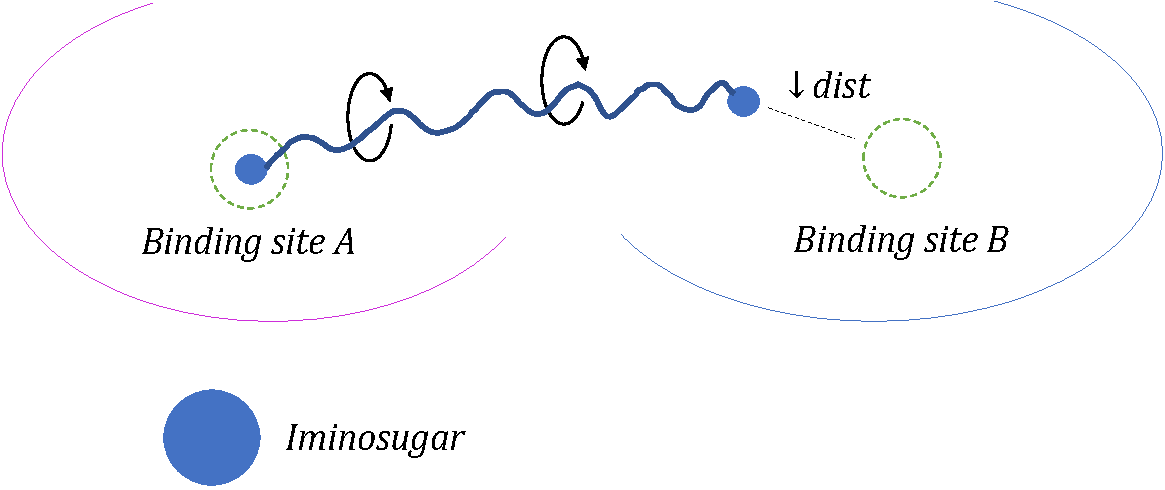
\includegraphics[width=\textwidth]{./figures/06/one-divalent-stretch-crop.pdf}
	\end{Center}
	\caption[Single di-ONJ inhibitor test]{To assess if a single divalent ONJ ligand can reach both binding sites of TmGH1 simultaneously, one iminosugar end was fixed in the binding site of one monomer (left) and the other end was instructed to minimize its distance to the other binding site (right) by exploring the free-torsion bonds rotation.}
	\label{fig:one-divalent-stretch}
\end{figure}



The results of this preliminary calculation confirmed that the synthesized divalent ligand was not long enough to reach the both sites. If one site was forced to be occupied by one of the iminosugars, the other end will stay at a distance of 12 \AA, even considering severe steric impediments. Seeing that a single divalent ligand cannot occupy both sites simultaneously, an inhibition mechanism by sliding is proposed. This is a, a single divalent molecule must be able to switch from one site to the other, taking advantage of having an iminosugar on both ends.

This observation makes the next question obvious: how long should it be then? The ligand is, simply put, two iminosugars connected by two chains of 10 atoms each. If we consider longer linkers, it might be possible to reach both. To assess that possibility, a library of linkers ranging from 13 to 16-carbon linear alkanes was constructed and the same protocol was applied, but changing the Molecule gene to consider a dynamic construction of molecules as explained in \autoref[section]{section:dibiotin-linker-length-optimization} (see fig. \ref{fig:divalent-length}). This can be set up by building this directory hierarchy:

\todo[inline]{Might be not necessary - consider appendix}

\begin{itemize}
	\item Dynamic-ligand/

\begin{itemize}
	\item 01-iminosugar/

\begin{itemize}
	\item Iminosugar-a.mol2


\end{itemize}
	\item 02-linker/

\begin{itemize}
	\item alkane-12.mol2, alkane-13C.mol2, $ \ldots $ , alkane-16C.mol2


\end{itemize}
	\item 03-connector/

\begin{itemize}
	\item T-connector.mol2


\end{itemize}
	\item 04-linker/

\begin{itemize}
	\item alkane-12.mol2, alkane-13C.mol2, $ \ldots $ , alkane-16C.mol2


\end{itemize}
	\item 05-iminosugar/

\begin{itemize}
	\item Iminosugar-b.mol2
\end{itemize}
\end{itemize}
\end{itemize}



\begin{figure}[H] % FIXME!
	\begin{Center}
		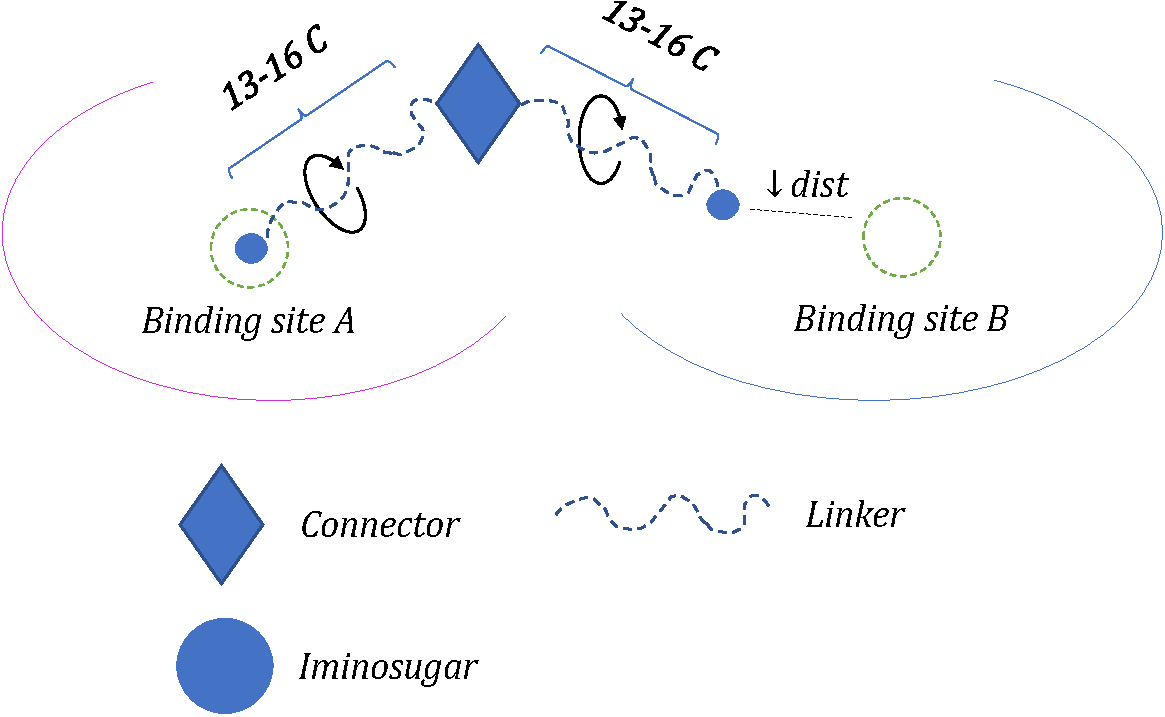
\includegraphics[width=\textwidth]{./figures/06/divalent-fragments-stretch-crop.pdf}
	\end{Center}
	\caption[Di-ONJ linker length optimization]{To guess the optimum length of the divalent linker, GaudiMM was instructed to build ligands with linkers ranging from 13 to 16 carbon atoms, explore their free-torsion bonds rotations and minimize the distance to binding site B.}
	\label{fig:divalent-length}
\end{figure}

The resulting ligand is always a linear concatenation iminosugar-linker-connector-linker-iminosugar compound, whose total length depends on the selected linkers. Again, for synthesis easiness, \textit{02-linker} and \textit{04-linker} fragments were set to be symmetric: they will always list the same alkane. The evaluation part is still the same: the non-frozen iminosugar will be forced to reach the other dimer, but only long enough ligands will be able to do so. The results show that linkers longer than 13 carbons are able to reach both sites comfortably without the need to slide from one to the other.

\subsubsection{Can two divalent ligands occupy both sites simultaneously? Do they interact?}
% \addcontentsline{toc}{subsubsection}{Can two divalent ligands occupy both sites simultaneously? Do they interact?}
A second hypothesis would consist of considering that two divalent ligands can occupy both sites of the same dimer simultaneously. If that is the case, they could even stabilize each other by interacting at the dimer interface via their free iminosugar moieties (which can form hydrogen bonds through their hydroxyl groups) or the coupling of their hydrophobic tails.

To assess that possibility, two molecules were superposed against the crystallographic binding sites of the dimer structure contained in PDB ID 2WBG, which features an analog inhibitor compound suitable for structural alignment. Then, dihedral torsions of the rotatable bonds of the ligand were analyzed looking for a combination that could have them interact at the interface. This interaction was implemented as a distance minimization between a carboxylic oxygen of one ligand and a carboxylic hydrogen of the other (see table \ref{table:recipe-two-divalent} and fig. \ref{fig:divalent-interface}).

\begin{table}[hbtp]
	\caption{Recipe used in the evaluation of a two di-ONJ ligands. The ligand wass positioned in such a way that one of the terminal iminosugars matched the crystallographic structure sof the ligand in the original 2WBG protein structure}
	\label{table:recipe-two-divalent}
	\footnotesize
	\newcolumntype{R}{>{\hsize=.25\hsize\raggedleft\arraybackslash}X}%
	\newcolumntype{L}{>{\hsize=.75\hsize\raggedright\arraybackslash}X}%
	\newcommand{\tableheading}[1]{\multicolumn{2}{c}{\textsc{#1}}}
	\begin{tabularx}{\textwidth}{RL}
		\toprule
		%row no:1
		\tableheading{Genes}\\
		\toprule
		%row no:2
		\texttt{Molecule} & Load the protein model obtained after cleaning the PDB structure \texttt{2WBG} (waters and ligands removed) \\
		\midrule
		%row no:3
		\texttt{Molecule} & Load one copy ligand using a Mol2 file obtained with ChemCraft, positioned in binding site of monomer A \\
		\midrule
		\texttt{Molecule} & Load another ligand using a Mol2 file obtained with ChemCraft, positioned in binding site of monomer B \\
		\midrule
		\texttt{Torsion} & Explore the free rotations of the ligand copy A. \\
		\midrule
		\texttt{Torsion} & Explore the free rotations of the ligand copy B. \\
		\toprule
		%row no:4
		\tableheading{Objectives}\\
		\toprule
		%row no:5
		\texttt{Contacts} & Minimize steric clashes \\
		\midrule
		%row no:6
		\texttt{Distance} & Bring the free iminosugar ends of both ligand copies close together so they are able to form a H-bond \\

		\bottomrule

	\end{tabularx}
\end{table}


\begin{figure} % FIXME!
	\begin{Center}
		\includegraphics[width=\textwidth]{./figures/06/divalent-interface-meeting.png}
	\end{Center}
	\caption[Dual di-ONJ interface meeting test]{Two divalent ONJ models were anchored to their respective binding sites, and their free-torsion bonds were explored to find a pose were the two free iminosugar ends could interact at the interface via a H-bond.}
	\label{fig:divalent-interface}
\end{figure}


The analysis showed that this interaction is structurally feasible, which was further confirmed by an explicitly solvated, full-atom molecular dynamics trajectory: the interaction remained stable for more than 100 nanoseconds. Simulating this system (100,000+ atoms) for such a long period of time can take months with ordinary CPUs, but thanks to the GPU acceleration implemented in OpenMM and OMMProtocol, these trajectories could be obtained within a week. An equivalent protocol in the commercial, GPU-accelerated version of Amber usually takes two weeks.

While the computational model offers an answer to whether this structure is possible of not, this specific protocol cannot answer whether this interaction is favored. To assess that possibility, broader sampling would be needed: metadynamics, replica exchange, free energy perturbation$ \ldots $  In fact, there is no experimental information to support this hypothetic interaction: the stoichiometry suggested leans towards 1:1, and not 2:1.

\subsubsection{Does the rotaxane compound fit? Can it occupy both sites? How?}
% \addcontentsline{toc}{subsubsection}{Does the rotaxane compound fit? Can it occupy both sites? How?}
The pillar[5]ene variants exhibit a slightly worse $K_{i}$ but still comparable to the di-ONJ compound, so one would expect a similar interaction profile. The divalent ligand has been shown that it cannot reach both sites of a dimer, suggesting that its inhibition mechanism is based on a sliding motion. However, the divalent ligand only represents half of the H-shaped component of the rotaxane compound. This has two conflicting consequences: (1) the H-shaped component is larger and could use the iminosugars of opposed axels to reach both binding sites, and (2) the crown component adds a volume that might work against this interaction through steric impediment. This raises two possibilities:

\begin{enumerate}
	\item The rotaxane interacts with the protein via iminosugars on the \textbf{same} axel.
	\begin{enumerate}
		\item This interaction strategy does not offer any advantage over the divalent binding (its iminosugar-iminosugar range distance is the same).
		\item The steric impediments of the crown component are easier to solve, since rest of the structure would remain facing the outside part of the structure.
	\end{enumerate}
	\item The rotaxane interacts with the protein via iminosugars on \textbf{different} axels.
	\begin{enumerate}
		\item The iminosugar-iminosugar range distance is far greater and could enable accessing both sites simultaneously.
		\item The steric impediments of the crown are far greater, since the structure would be now in a less ideal orientation.
	\end{enumerate}
\end{enumerate}

To assess both possibilities, the protein-rotaxane structure was analysed with GaudiMM following the same recipe as the single divalent molecule docking in \autoref[section]{section:di-ONJ-stretch}: one iminosugar was fixed in one binding site and the second one was instructed to get close to the second binding site with a distance minimization objective by exploring the free torsion of rotatable bonds. Steric clashes were minimized through a Contacts objective. See table \ref{table:recipe-rotaxane} for more details.

In the binding mode A (same axel), the structure did not reach the second binding site, as expected; not even tolerating severe clashes. In binding mode B (different axels), the H-shaped component could reach both sites comfortably. There were clashes, but not as bad as expected: they were mainly due to internal clashes of the rotaxane. Given the unusually high number of freely rotatable bonds (176 in this case), more iterations would have been needed to optimize them out. However, that was not necessary, since the purpose of these GaudiMM calculations was to obtain a \textit{good enough} structure to use as the starting point of the next step in the multiscale protocol.


\begin{table}[hbtp]
	\caption{Recipe used in the evaluation of the pillar[5]ene ligand. The ligand wass positioned in such a way that one of the terminal iminosugars matched the crystallographic structure of the ligand in one of the monomers of the original 2WBG protein structure.}
	\label{table:recipe-rotaxane}
	\footnotesize
	\newcolumntype{R}{>{\hsize=.25\hsize\raggedleft\arraybackslash}X}%
	\newcolumntype{L}{>{\hsize=.75\hsize\raggedright\arraybackslash}X}%
	\newcommand{\tableheading}[1]{\multicolumn{2}{c}{\textsc{#1}}}
	\begin{tabularx}{\textwidth}{RL}
		\toprule
		%row no:1
		\tableheading{Genes}\\
		\toprule
		%row no:2
		\texttt{Molecule} & Load the protein model obtained after cleaning the PDB structure \texttt{2WBG} (waters and ligands removed) \\
		\midrule
		%row no:3
		\texttt{Molecule} & Load the structure of the pillar[5]ene as obtained through a preliminary 3D model in ChemCraft \\
		\midrule
		\texttt{Torsion} & Explore the free rotations of the pillar[5]ene. \\
		\toprule
		%row no:4
		\tableheading{Objectives}\\
		\toprule
		%row no:5
		\texttt{Contacts} & Minimize steric clashes \\
		\midrule
		%row no:6
		\texttt{Distance} & Bring one of the free iminosugar ends (depending on the case studied, from the same axel or from the one across) closer to the binding site in monomer B \\

		\bottomrule

	\end{tabularx}
\end{table}

Once parameterized, two candidate structures of each binding mode were submitted to a molecular dynamics analysis with OMMProtocol. Both revealed stable bindings to their respective sites, with additional stabilization of the structure via internal cross-interactions.

The unsurprising results observed for binding mode A (same axel) agree with the experimental evidences. It exhibits the same binding profile as a single divalent molecule, compatible with the sliding mechanism, hence the comparable Ki values. The slight difference might be due to \todo{the entropic stabilization} of the crown-component via secondary binding sites.

Unfortunately, while the binding mode B (different axels) showed a promising interaction profile, there is no experimental evidence to back it up. If this binding mode was feasible, a higher Ki should be observed, but that is not the case.

\subsection{Discussion \& Further work}
% \addcontentsline{toc}{subsection}{Discussion $\&$  Further work}
This joint study was an excellent opportunity to prove how GaudiMM has proved can be a valuable asset for both experimental and computational communities. The computational feedback has provided illustrative models on what can be happening at the molecular level and even proposed alternative explanations to be confirmed experimentally. This can be argued in three points.

First, GaudiMM can provide results directly applicable to the wet-lab. The different di-ONJ variants tested opened doors to synthesizing ligands of optimum length that would explain how the di-ONJ ligand exhibits that excellent inhibition power without incurring in additional costs. Doing this experimentally would have involved more steps of synthesis and tests, only to discard most of the candidate ligands. With this computational framework, this can be obtained within a day. Of course, this does not replace the experimental data; it just reflects that computational assessment can at least provide a way to save some money from the increasingly tight budgets, both in materials and human work.

Second, it allows to create new types of computational studies in a simpler, consistent way. Testing if the di-ONJ compound or the rotaxane can reach both binding sites of a dimeric protein would be normally done with a steered molecular dynamics simulation. However, parameterization would be needed first. For the rotaxane alone, this would take more than a day. The actual simulation would take around a week. With GaudiMM, this can be obtained in hours. Then, if the results are positive, a MD simulation would be in order. However, if the results did not show anything promising, those expensive computational and time resources could be invested in testing a different hypothesis. In the same fashion, testing if two divalent ONJ ligands can interact at the interface would be usually studied with molecular docking, but there is no software suite that can perform a multi-ligand, restrained study like the one herein presented.

Third, even if the researchers prefer to go straight to the MD stage without confirming the feasibility of the hypothesis first, they would still need to build the initial structure first. The researcher usually constructs those manually, with the aid of an interactive 3D viewer and related tools. This is normally doable with small ligands, but it starts getting disturbingly complex when bigger structures are involved. Setting up a rotaxane model suitable for MD assessment would have involved hours of finetuning and trial-and-error attempts. With GaudiMM, these can be obtained automatically when the correct recipe is used.

Of course, GaudiMM is not the answer to every question. It only helps guide the creation of new hypothesis at the initial steps of the brainstorming. For more accurate results, higher levels of theory must be applied through more advanced protocols. Even molecular dynamics might not be enough if quantitative magnitudes are demanded, such as binding energy or free energy. To obtain those, one would have to employ broad sampling methods like metadynamics or free energy perturbation, hybrid schemes like QM/MM, or even QM calculations of reduced cluster models. Those are out the scope of this dissertation and could not be performed within the available timeframe.

\section{Final conclusions}
% \addcontentsline{toc}{section}{Final conclusions}
Throughout this chapter, it has been shown that, while computational studies can be strictly theoretical, there is no point in denying that molecular modeling is a helpful tool for experimental works. \textit{In silico} can go hand in hand with \textit{in vitro}, and some research groups would argue that they must. It is common to see how experimental groups maintain strong alliances with theoretical groups, and some are even creating their own computational shops within their established wet-lab structure \todo{Citations needed}. Fruitful joint efforts like this bring different points of view and ways of thinking to the discussion table, which can only enhance the brainstorming sessions, especially when counterintuitive phenomena like the aforementioned happen.

